\chapter{Simulaciones}
\lhead{\emph{Simulaciones}}

En este capítulo se presentan las mediciones y ensayos realizados para estudiar y comparar como se comportan ambos métodos de
calibración, clásica y utilizando acoplamientos mútuos.

La configuración de la antena a utilizar para todos los ensayos está especificada en la tabla \ref{tab:configurationUsed} y 
consta de 70 elementos radiantes. Las especificaciones de las propiedades físicas de cada componente están definidas en la 
tabla \ref{tab:configurationOfComponents}.
\begin{table}[H]
  \footnotesize
  \centering
  \begin{tabular}{|c|c|}
	\hline
	\textbf{Componente de Antena} & \textbf{Configuración} \tabularnewline \hline 
	freq &  1275000000 [Hz] \tabularnewline\hline 
	power & 0 [dB] \tabularnewline \hline 
	phase & 0 [deg] \tabularnewline \hline 
	desiredTxPower & 6 [dB] \tabularnewline \hline 
	desiredRxPower & 0 [dB] \tabularnewline \hline 
	quantityRows & 7 \tabularnewline \hline 
	quantityColumns & 10 \tabularnewline \hline 
	verticalSeparation & 0.2 [m] \tabularnewline \hline 
	hotizontalSeparation & 0.2 [m] \tabularnewline \hline 
	componentSequence & [cable1, psc17, cable1, psc15, cable2, psc12, trm, circulator, cable3, rm] \tabularnewline \hline 
  \end{tabular}
  \caption{Configuración de la antena común para todos los ensayos.}
  \label{tab:configurationUsed}
\end{table}
\begin{table}[H]
  \footnotesize
  \centering
  \begin{tabular}{|c|c|c|}
	\hline
	\textbf{Componente de Antena} & \textbf{Cacarcterísticas físicas} & \textbf{Configuración} \tabularnewline \hline 
	\multirow{2}{*}{cable1} &  attenuation [db] & 0.1\tabularnewline \cline{2-3}
	 & length [m] & 0.45\tabularnewline \hline 
	\multirow{2}{*}{cable2} &  attenuation [db] & 0.1\tabularnewline \cline{2-3}
	 & length [m] & 8\tabularnewline \hline 
	\multirow{2}{*}{cable3} &  attenuation [db] & 0.1\tabularnewline \cline{2-3}
	 & length [m] & 0.5\tabularnewline \hline 
	psc17 & outputPorts & 7\tabularnewline \hline
	psc15 & outputPorts & 5\tabularnewline \hline
	psc12 & outputPorts & 2\tabularnewline \hline
	\multirow{2}{*}{TRM} & gain [db] & 10\tabularnewline \cline{2-3}
	 & phaseShift [deg] & 10\tabularnewline \hline 
	circulator & & \tabularnewline \hline 
	RM & & \tabularnewline \hline 
  \end{tabular}
  \caption{Configuración de las propiedades físicas de cada componente de la antena utilizada en todos los ensayos.}
  \label{tab:configurationOfComponents}
\end{table}
La numeración de los elementos tiene un orden de izquierda a derecha y de arriba hacia abajo, de tal forma que el elemnto cero 
es el superior izquierdo de la antena.

Para una mayor claridad, todos los gráficos representan cómo ambos métodos calibran la antena en un estado puntual. No se 
realizaron ensayos utilizando el método montecarlo dado que no se agregaron incertidumbres en el instrumento de medición de las 
distintas señales recibidas de los lazos de calibración.

Todos los ensayos de las siguientes secciones poseen las siguientes característicias:
\begin{itemize}
	\item Se utilizan diferentes apuntamientos de la antena. Los cuales son uniforme, 10 grados en la dirección horizontal y 10 
		grados en la dirección vertical.
	\item Se muestra un gráfico de la potencia y fase transmitida para cada apuntamiento utilizado. En los cuales se observan las
		señales sin calibrar, calibrada e ideal. 
	\item Se grafican los patrones de antena para los cortes horizontal y vertical de las señales transmitidas sin calibrar, 
		calibradas e ideales.
\end{itemize}


\section{Sin dispersiones}

Los ensayos de esta sección tienen las siguientes caracterísiticas,
\begin{itemize}
	\item Los componentes de antena no tienen ningún prolema de funcionamiento ni hay desadaptaciones.
	\item No hay dispersiones de calibración.
	\item No hay dispersiones en la señal.
\end{itemize}

\subsection{Utilizando la calibración clásica}

En las figuras \ref{fig:nonErrClassical0deg}, \ref{fig:nonErrClassical10degCol} y \ref{fig:nonErrClassical10degRow} se muestran
los resultados de la calibración clásica con una antena sin dispersiones. Se puede apreciar que, si bien la antena tiene un 
comportamiento ideal, las mediciones no son completamente correctas. Dicha dispersión se debe a que el método no abarca la 
totalidad de la antena.


\subsubsection{Apuntamiento uniforme}

\begin{figure}[H]
	\centering
 	\subfloat[]{
		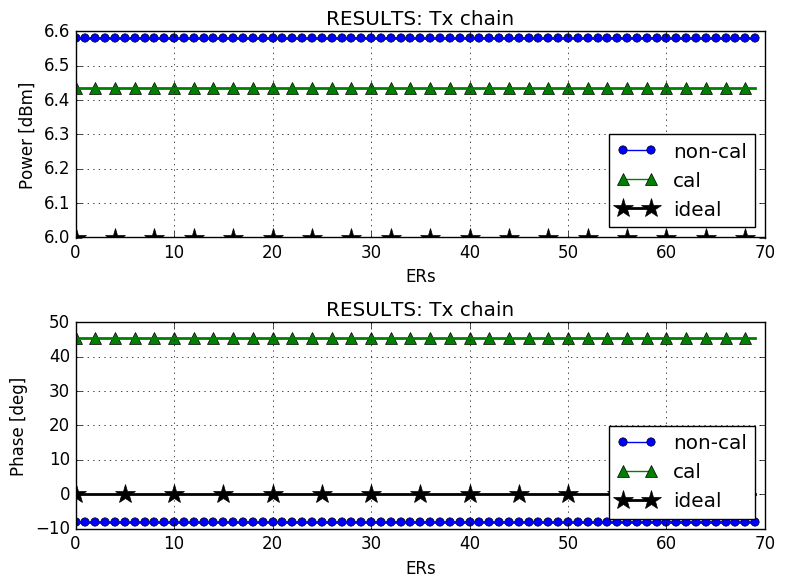
\includegraphics[width=10cm]{gfx/nonErrClassical0deg.png}}

	\subfloat[]{
		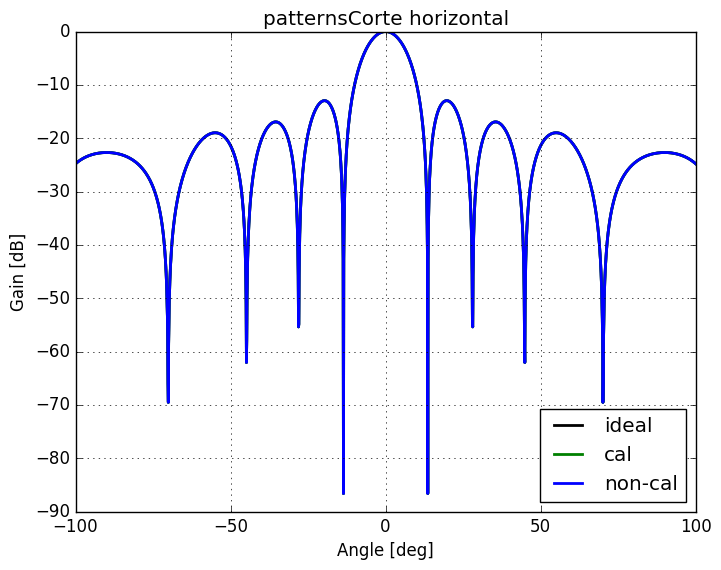
\includegraphics[width=8cm]{gfx/nonErrClassical0degAzCut.png}}
 	\subfloat[]{
		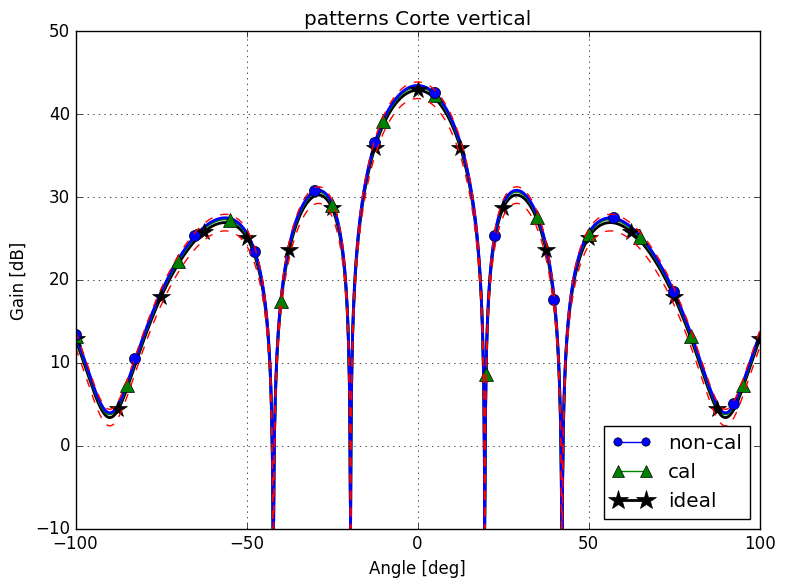
\includegraphics[width=8cm]{gfx/nonErrClassical0degElCut.png}}
	\caption{Correcciones de la señal transmitida utilizando calibración clásica. (a) ganancia y fase transmitida por módulos
		radiantes. (b) corte horizontal del patrón transmitido y (c) corte vertical del patrón transmitido.}
	\label{fig:nonErrClassical0deg}
\end{figure}

\begin{table}[H]
  \footnotesize
  \centering
  \begin{tabular}{|c|c|p{2cm}|p{2cm}|p{2cm}|p{2cm}|}
    \cline{2-6}
    \multicolumn{1}{c|}{} & \textbf{Corte} & \textbf{Potencia - lóbulo izquierdo} & \textbf{Potencia - lóbulo central} &
    \textbf{Potencia - lóbulo derecho} & \textbf{Ancho - lóbulo central} \tabularnewline\hline
    \multirow{2}{*}{\textbf{patrón sin calibrar}} & H & 26.37 & 39.34 & 26.37 & 12.0 \tabularnewline\cline{2-6}
     & V & 30.83 & 43.48 & 30.83 & 17.8 \tabularnewline\hline
    \multirow{2}{*}{\textbf{Patrón calibrada}} & H & 26.22 & 39.19 & 26.22 & 12.0 \tabularnewline\cline{2-6}
     & V & 30.68 & 43.34 & 30.68 & 17.8 \tabularnewline\hline
    \multirow{2}{*}{\textbf{Patrón ideal}} & H & 25.79 & 38.76 & 25.79 & 12.0 \tabularnewline\cline{2-6}
     & V & 30.25 & 42.9 & 30.25 & 17.8 \tabularnewline\hline
    \multirow{2}{*}{\textbf{Diferencia sin calibrar}} & H & 0.58 & 0.58 & 0.58 & 0.0\tabularnewline\cline{2-6}
     & V & 0.58 & 0.58 & 0.58 & 0.0 \tabularnewline\hline
    \multirow{2}{*}{\textbf{Diferencia calibrada}} & H & 0.43 & 0.43 & 0.43 & 0.0 \tabularnewline\cline{2-6}
     & V & 0.43 & 0.44 & 0.43 & 0.0 \tabularnewline\hline
  \end{tabular}
  \caption{Propiedades de los patrones calibrados y sin calibrar comparados con el ideal.}
  \label{tab:nonErrClassical0deg}
\end{table}


\subsubsection{Apuntamiento 10 grados en dirección horizontal}

\begin{figure}[H]
	\centering
 	\subfloat[]{
		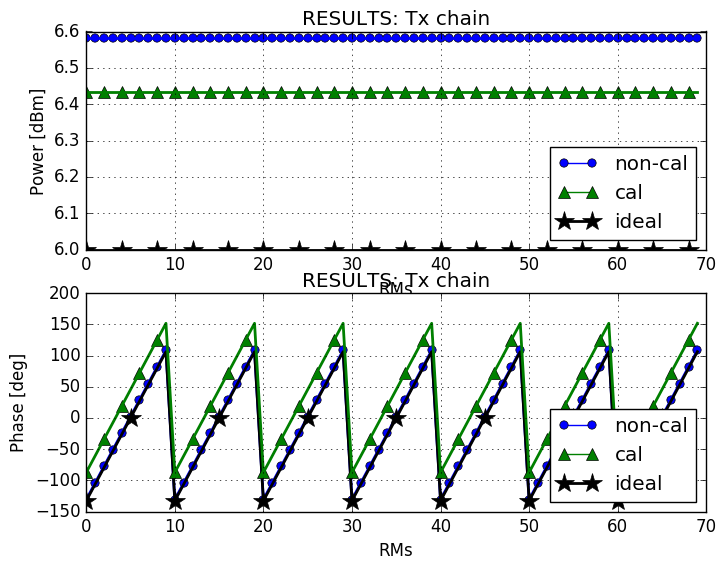
\includegraphics[width=10cm]{gfx/nonErrClassical10degCol.png}}

	\subfloat[]{
		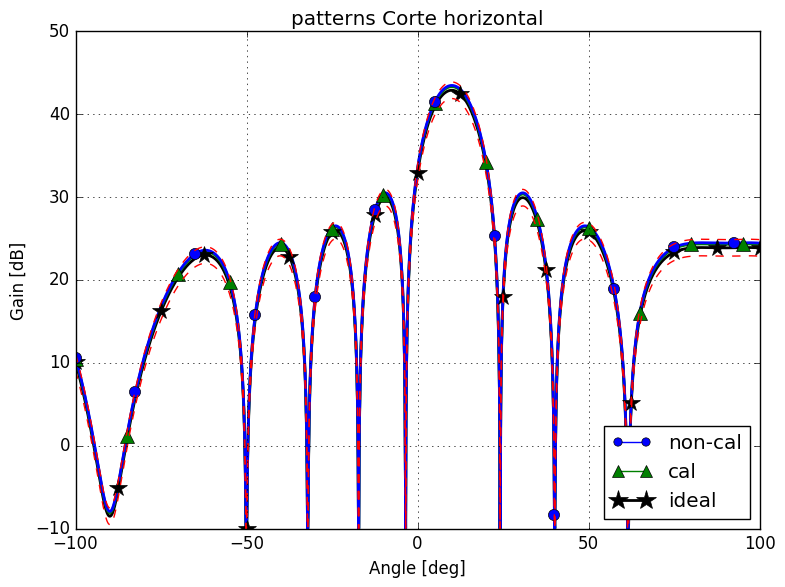
\includegraphics[width=8cm]{gfx/nonErrClassical10degColAzCut.png}}
 	\subfloat[]{
		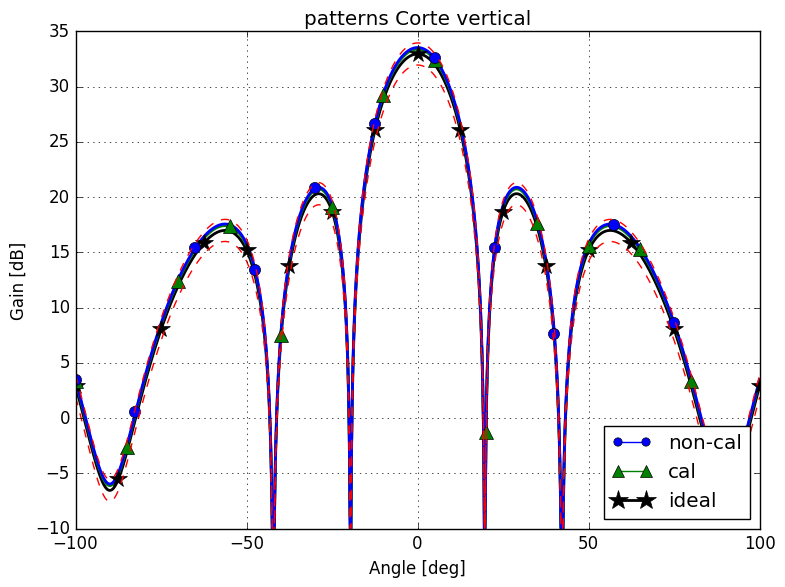
\includegraphics[width=8cm]{gfx/nonErrClassical10degColElCut.png}}
	\caption{Correcciones de la señal transmitida utilizando calibración clásica. (a) ganancia y fase transmitida por módulos
		radiantes. (b) corte horizontal del patrón transmitido y (c) corte vertical del patrón transmitido.}
	\label{fig:nonErrClassical10degCol}
\end{figure}

\begin{table}[H]
  \footnotesize
  \centering
  \begin{tabular}{|c|c|p{2cm}|p{2cm}|p{2cm}|p{2cm}|}
    \cline{2-6}
    \multicolumn{1}{c|}{} & \textbf{Corte} & \textbf{Potencia - lóbulo izquierdo} & \textbf{Potencia - lóbulo central} &
    \textbf{Potencia - lóbulo derecho} & \textbf{Ancho - lóbulo central} \tabularnewline\hline
    \multirow{2}{*}{\textbf{patrón sin calibrar}} & H & 26.37 & 39.34 & 26.37 & 12.0 \tabularnewline\cline{2-6}
     & V & 30.83 & 43.48 & 30.83 & 17.8 \tabularnewline\hline
    \multirow{2}{*}{\textbf{Patrón calibrada}} & H & 26.22 & 39.19 & 26.22 & 12.0 \tabularnewline\cline{2-6}
     & V & 30.68 & 43.34 & 30.68 & 17.8 \tabularnewline\hline
    \multirow{2}{*}{\textbf{Patrón ideal}} & H & 25.79 & 38.76 & 25.79 & 12.0 \tabularnewline\cline{2-6}
     & V & 30.25 & 42.9 & 30.25 & 17.8 \tabularnewline\hline
    \multirow{2}{*}{\textbf{Diferencia sin calibrar}} & H & 0.58 & 0.58 & 0.58 & 0.0\tabularnewline\cline{2-6}
     & V & 0.58 & 0.58 & 0.58 & 0.0 \tabularnewline\hline
    \multirow{2}{*}{\textbf{Diferencia calibrada}} & H & 0.43 & 0.43 & 0.43 & 0.0 \tabularnewline\cline{2-6}
     & V & 0.43 & 0.44 & 0.43 & 0.0 \tabularnewline\hline
  \end{tabular}
  \caption{Propiedades de los patrones calibrados y sin calibrar comparados con el ideal.}
  \label{tab:nonErrClassical10degCol}
\end{table}


\subsubsection{Apuntamiento 10 grados en dirección vertical}

\begin{figure}[H]
	\centering
 	\subfloat[]{
		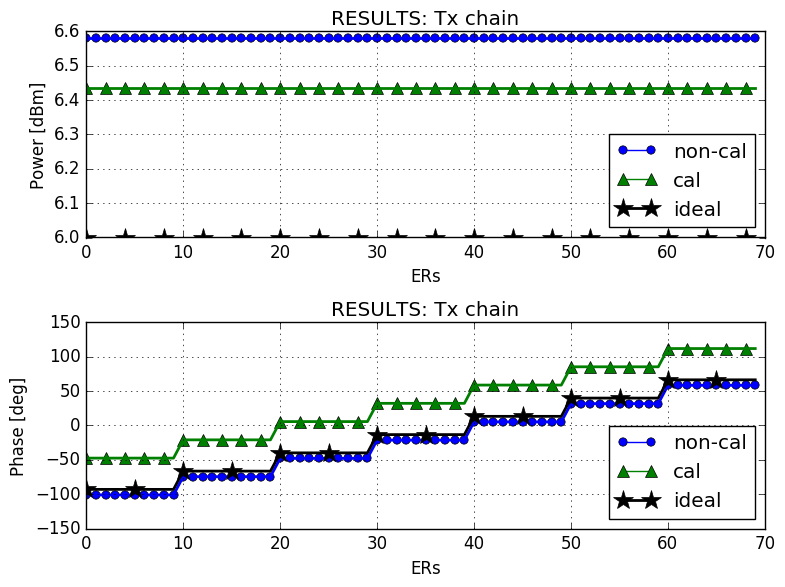
\includegraphics[width=10cm]{gfx/nonErrClassical10degRow.png}}

	\subfloat[]{
		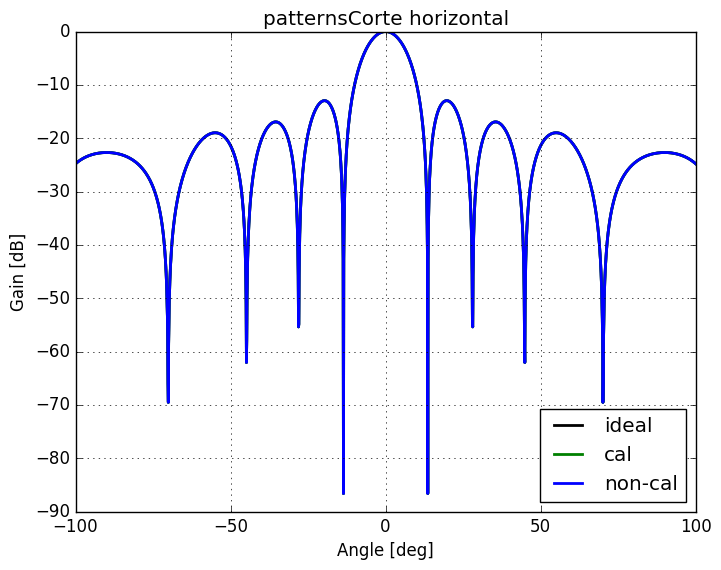
\includegraphics[width=8cm]{gfx/nonErrClassical10degRowAzCut.png}}
 	\subfloat[]{
		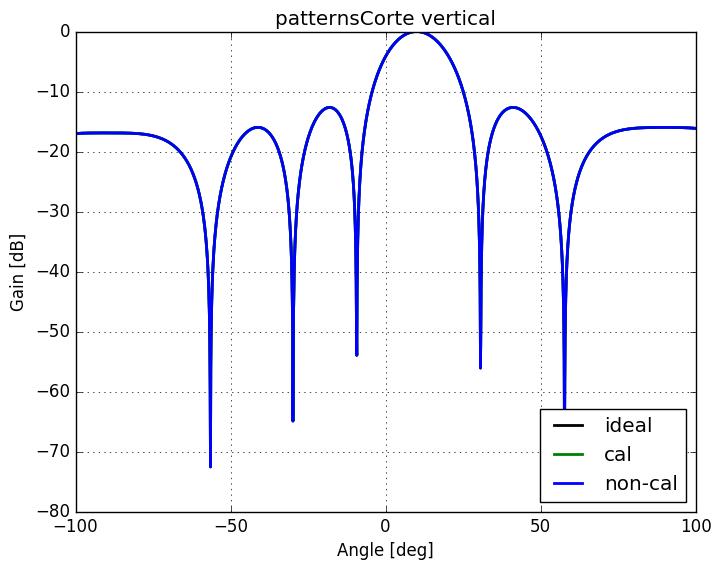
\includegraphics[width=8cm]{gfx/nonErrClassical10degRowElCut.png}}
	\caption{Correcciones de la señal transmitida utilizando calibración clásica. (a) ganancia y fase transmitida por módulos
		radiantes. (b) corte horizontal del patrón transmitido y (c) corte vertical del patrón transmitido.}
	\label{fig:nonErrClassical10degRow}
\end{figure}

\begin{table}[H]
  \footnotesize
  \centering
  \begin{tabular}{|c|c|p{2cm}|p{2cm}|p{2cm}|p{2cm}|}
    \cline{2-6}
    \multicolumn{1}{c|}{} & \textbf{Corte} & \textbf{Potencia - lóbulo izquierdo} & \textbf{Potencia - lóbulo central} &
    \textbf{Potencia - lóbulo derecho} & \textbf{Ancho - lóbulo central} \tabularnewline\hline
    \multirow{2}{*}{\textbf{patrón sin calibrar}} & H & 26.37 & 39.34 & 26.37 & 12.0 \tabularnewline\cline{2-6}
     & V & 30.83 & 43.48 & 30.83 & 17.8 \tabularnewline\hline
    \multirow{2}{*}{\textbf{Patrón calibrada}} & H & 26.22 & 39.19 & 26.22 & 12.0 \tabularnewline\cline{2-6}
     & V & 30.68 & 43.34 & 30.68 & 17.8 \tabularnewline\hline
    \multirow{2}{*}{\textbf{Patrón ideal}} & H & 25.79 & 38.76 & 25.79 & 12.0 \tabularnewline\cline{2-6}
     & V & 30.25 & 42.9 & 30.25 & 17.8 \tabularnewline\hline
    \multirow{2}{*}{\textbf{Diferencia sin calibrar}} & H & 0.58 & 0.58 & 0.58 & 0.0\tabularnewline\cline{2-6}
     & V & 0.58 & 0.58 & 0.58 & 0.0 \tabularnewline\hline
    \multirow{2}{*}{\textbf{Diferencia calibrada}} & H & 0.43 & 0.43 & 0.43 & 0.0 \tabularnewline\cline{2-6}
     & V & 0.43 & 0.44 & 0.43 & 0.0 \tabularnewline\hline
  \end{tabular}
  \caption{Propiedades de los patrones calibrados y sin calibrar comparados con el ideal.}
  \label{tab:nonErrClassical10degRow}
\end{table}


\subsection{Utilizando la calibración con acoplamientos mútuos}


\subsubsection{Apuntamiento uniforme}

\begin{figure}[H]
	\centering
 	\subfloat[]{
		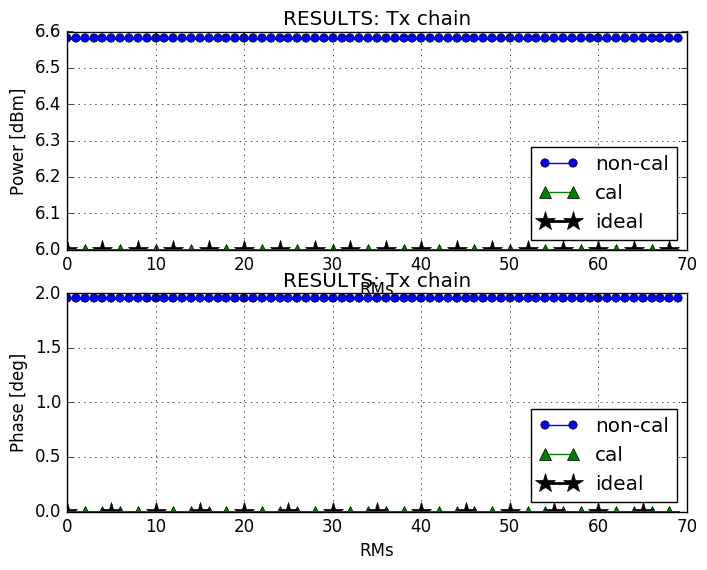
\includegraphics[width=10cm]{gfx/nonErrMutual0deg.png}}

	\subfloat[]{
		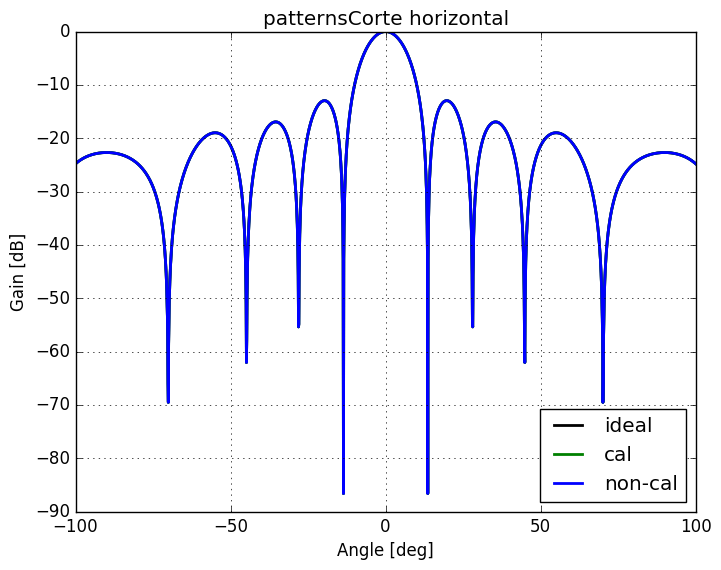
\includegraphics[width=8cm]{gfx/nonErrMutual0degAzCut.png}}
 	\subfloat[]{
		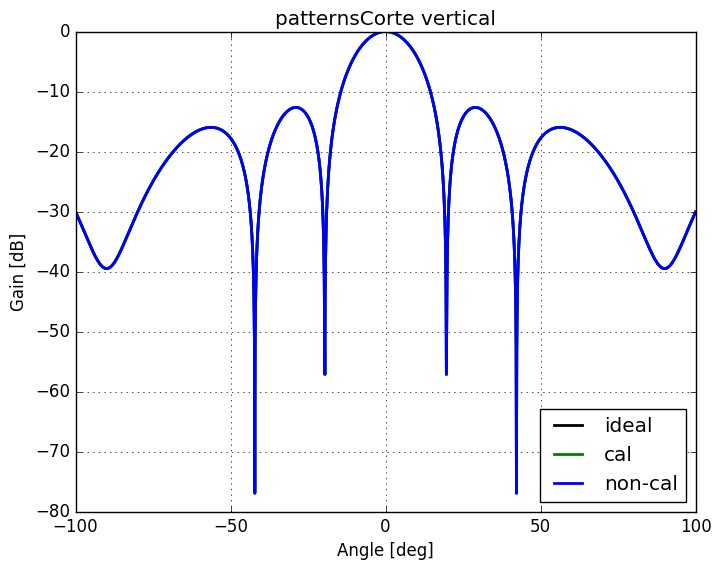
\includegraphics[width=8cm]{gfx/nonErrMutual0degElCut.png}}
	\caption{Correcciones de la señal transmitida utilizando calibración por acoplamientos mutuos. (a) ganancia y fase transmitida por módulos
		radiantes. (b) corte horizontal del patrón transmitido y (c) corte vertical del patrón transmitido.}
	\label{fig:nonErrMutual0deg}
\end{figure}

\begin{table}[H]
  \footnotesize
  \centering
  \begin{tabular}{|c|c|p{2cm}|p{2cm}|p{2cm}|p{2cm}|}
    \cline{2-6}
    \multicolumn{1}{c|}{} & \textbf{Corte} & \textbf{Potencia - lóbulo izquierdo} & \textbf{Potencia - lóbulo central} &
    \textbf{Potencia - lóbulo derecho} & \textbf{Ancho - lóbulo central} \tabularnewline\hline
    \multirow{2}{*}{\textbf{patrón sin calibrar}} & H & 26.37 & 39.34 & 26.37 & 12.0 \tabularnewline\cline{2-6}
     & V & 30.83 & 43.48 & 30.83 & 17.8 \tabularnewline\hline
    \multirow{2}{*}{\textbf{Patrón calibrada}} & H & 26.22 & 39.19 & 26.22 & 12.0 \tabularnewline\cline{2-6}
     & V & 30.68 & 43.34 & 30.68 & 17.8 \tabularnewline\hline
    \multirow{2}{*}{\textbf{Patrón ideal}} & H & 25.79 & 38.76 & 25.79 & 12.0 \tabularnewline\cline{2-6}
     & V & 30.25 & 42.9 & 30.25 & 17.8 \tabularnewline\hline
    \multirow{2}{*}{\textbf{Diferencia sin calibrar}} & H & 0.58 & 0.58 & 0.58 & 0.0\tabularnewline\cline{2-6}
     & V & 0.58 & 0.58 & 0.58 & 0.0 \tabularnewline\hline
    \multirow{2}{*}{\textbf{Diferencia calibrada}} & H & 0.43 & 0.43 & 0.43 & 0.0 \tabularnewline\cline{2-6}
     & V & 0.43 & 0.44 & 0.43 & 0.0 \tabularnewline\hline
  \end{tabular}
  \caption{Propiedades de los patrones calibrados y sin calibrar comparados con el ideal.}
  \label{tab:nonErrMutual0deg}
\end{table}


\subsubsection{Apuntamiento 10 grados en dirección horizontal}

\begin{figure}[H]
	\centering
 	\subfloat[]{
		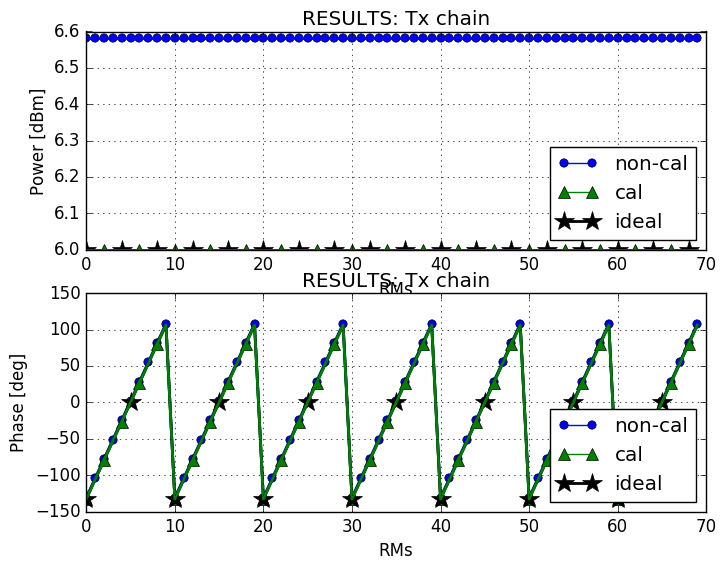
\includegraphics[width=10cm]{gfx/nonErrMutual10degCol.png}}

	\subfloat[]{
		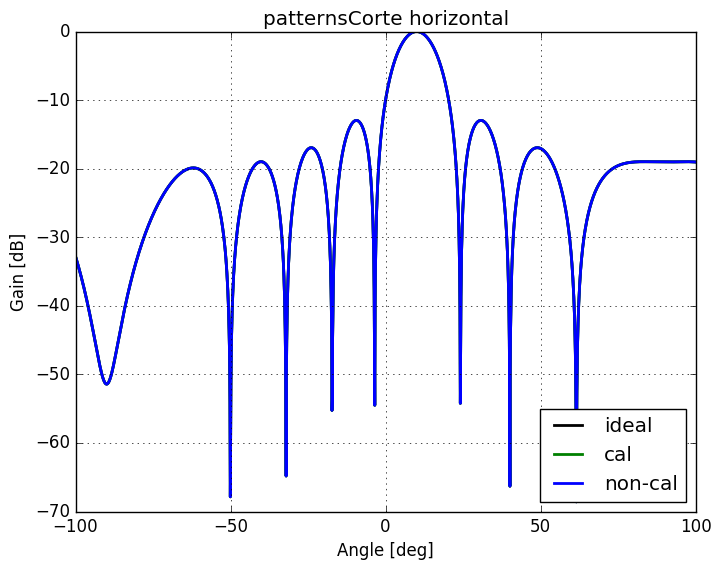
\includegraphics[width=8cm]{gfx/nonErrMutual10degColAzCut.png}}
 	\subfloat[]{
		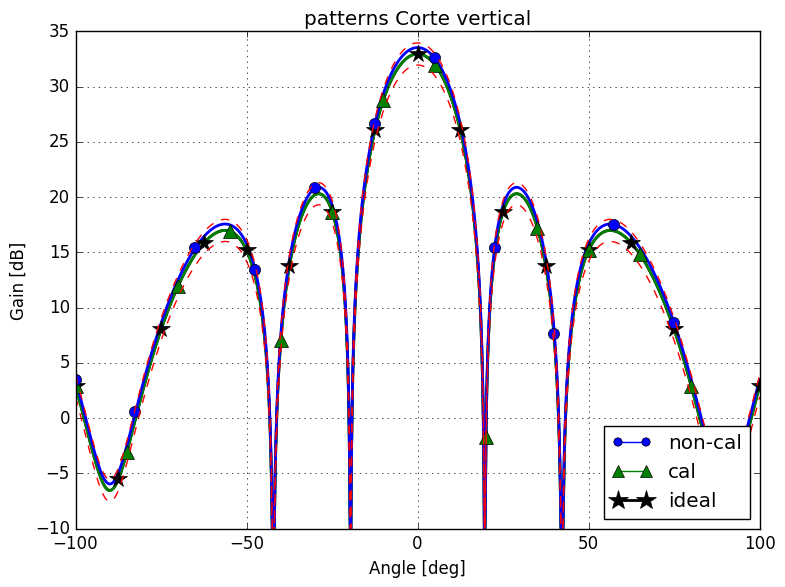
\includegraphics[width=8cm]{gfx/nonErrMutual10degColElCut.png}}
	\caption{Correcciones de la señal transmitida utilizando calibración por acoplamientos mutuos. (a) ganancia y fase 
		transmitida por módulos radiantes. (b) corte horizontal del patrón transmitido y (c) corte vertical del patrón transmitido.}
	\label{fig:nonErrMutual10degCol}
\end{figure}

\begin{table}[H]
  \footnotesize
  \centering
  \begin{tabular}{|c|c|p{2cm}|p{2cm}|p{2cm}|p{2cm}|}
    \cline{2-6}
    \multicolumn{1}{c|}{} & \textbf{Corte} & \textbf{Potencia - lóbulo izquierdo} & \textbf{Potencia - lóbulo central} &
    \textbf{Potencia - lóbulo derecho} & \textbf{Ancho - lóbulo central} \tabularnewline\hline
    \multirow{2}{*}{\textbf{patrón sin calibrar}} & H & 26.37 & 39.34 & 26.37 & 12.0 \tabularnewline\cline{2-6}
     & V & 30.83 & 43.48 & 30.83 & 17.8 \tabularnewline\hline
    \multirow{2}{*}{\textbf{Patrón calibrada}} & H & 26.22 & 39.19 & 26.22 & 12.0 \tabularnewline\cline{2-6}
     & V & 30.68 & 43.34 & 30.68 & 17.8 \tabularnewline\hline
    \multirow{2}{*}{\textbf{Patrón ideal}} & H & 25.79 & 38.76 & 25.79 & 12.0 \tabularnewline\cline{2-6}
     & V & 30.25 & 42.9 & 30.25 & 17.8 \tabularnewline\hline
    \multirow{2}{*}{\textbf{Diferencia sin calibrar}} & H & 0.58 & 0.58 & 0.58 & 0.0\tabularnewline\cline{2-6}
     & V & 0.58 & 0.58 & 0.58 & 0.0 \tabularnewline\hline
    \multirow{2}{*}{\textbf{Diferencia calibrada}} & H & 0.43 & 0.43 & 0.43 & 0.0 \tabularnewline\cline{2-6}
     & V & 0.43 & 0.44 & 0.43 & 0.0 \tabularnewline\hline
  \end{tabular}
  \caption{Propiedades de los patrones calibrados y sin calibrar comparados con el ideal.}
  \label{tab:nonErrMutual10degCol}
\end{table}


\subsubsection{Apuntamiento 10 grados en dirección vertical}

En la figuras \ref{fig:nonErrMutual10degRow} se puede verificar que el apuntamiento es el correcto por los defasajes observados, 
como hay 10 elementos radiantes por fila, al apuntar verticalmente, cada fila posee un defasaje diferente, es por esta razón que 
la tercer fila se ve un gráfico estilo una escalera con siete escalones (que es la cantidad de columnas de la antena). A su vez, 
se aprecia que el calibrador lleva tanto la potencia como la fase transmitida al valor deseado.
\begin{figure}[H]
	\centering
 	\subfloat[]{
		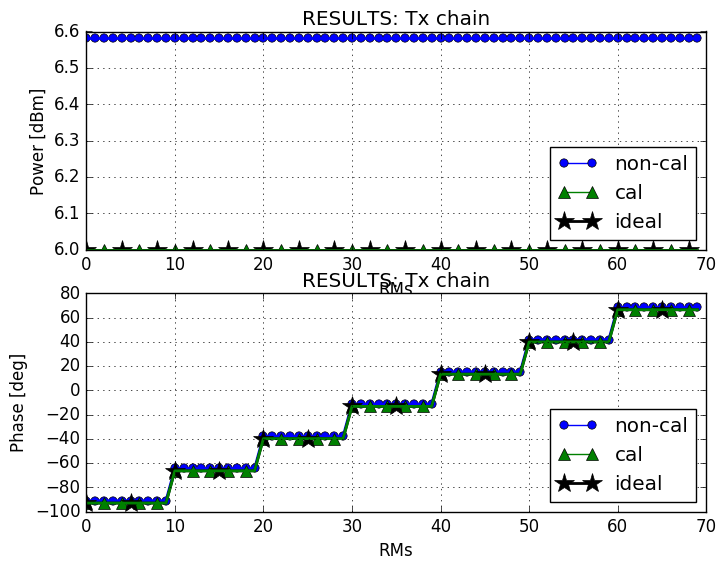
\includegraphics[width=10cm]{gfx/nonErrMutual10degRow.png}}

	\subfloat[]{
		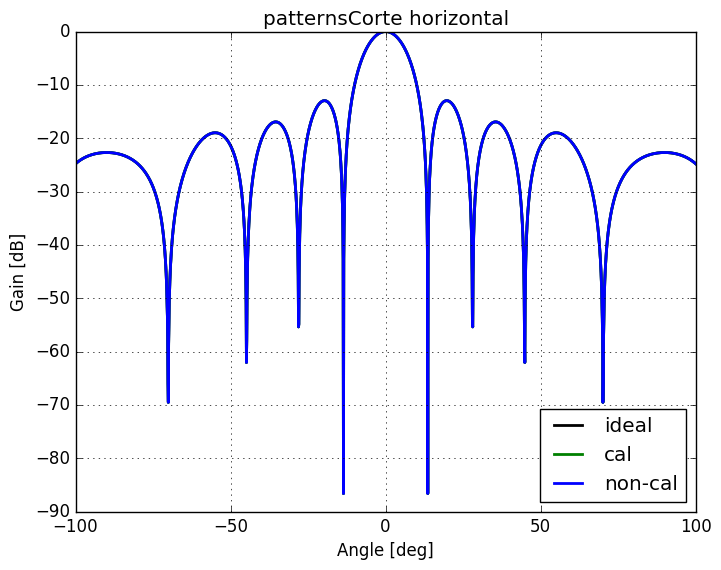
\includegraphics[width=8cm]{gfx/nonErrMutual10degRowAzCut.png}}
 	\subfloat[]{
		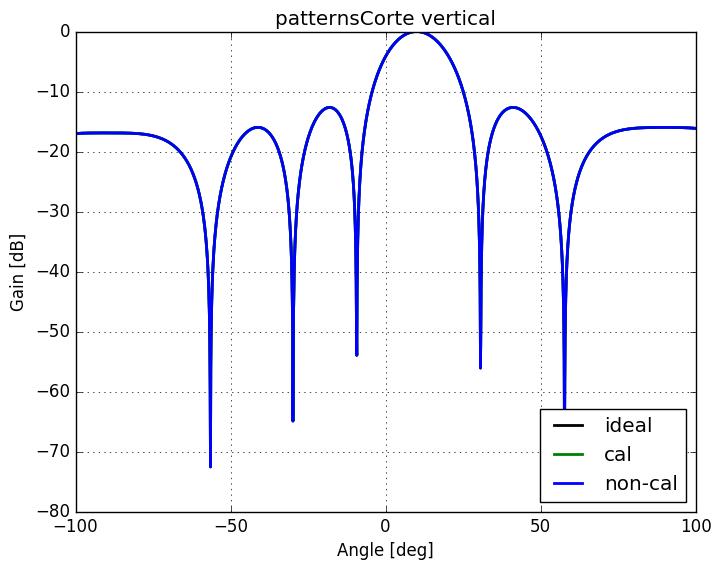
\includegraphics[width=8cm]{gfx/nonErrMutual10degRowElCut.png}}
	\caption{Correcciones de la señal transmitida utilizando calibración por acoplamientos mutuos. (a) ganancia y fase 
		transmitida por módulos radiantes. (b) corte horizontal del patrón transmitido y (c) corte vertical del patrón transmitido.}
	\label{fig:nonErrMutual10degRow}
\end{figure}

\begin{table}[H]
  \footnotesize
  \centering
  \begin{tabular}{|c|c|p{2cm}|p{2cm}|p{2cm}|p{2cm}|}
    \cline{2-6}
    \multicolumn{1}{c|}{} & \textbf{Corte} & \textbf{Potencia - lóbulo izquierdo} & \textbf{Potencia - lóbulo central} &
    \textbf{Potencia - lóbulo derecho} & \textbf{Ancho - lóbulo central} \tabularnewline\hline
    \multirow{2}{*}{\textbf{patrón sin calibrar}} & H & 26.37 & 39.34 & 26.37 & 12.0 \tabularnewline\cline{2-6}
     & V & 30.83 & 43.48 & 30.83 & 17.8 \tabularnewline\hline
    \multirow{2}{*}{\textbf{Patrón calibrada}} & H & 26.22 & 39.19 & 26.22 & 12.0 \tabularnewline\cline{2-6}
     & V & 30.68 & 43.34 & 30.68 & 17.8 \tabularnewline\hline
    \multirow{2}{*}{\textbf{Patrón ideal}} & H & 25.79 & 38.76 & 25.79 & 12.0 \tabularnewline\cline{2-6}
     & V & 30.25 & 42.9 & 30.25 & 17.8 \tabularnewline\hline
    \multirow{2}{*}{\textbf{Diferencia sin calibrar}} & H & 0.58 & 0.58 & 0.58 & 0.0\tabularnewline\cline{2-6}
     & V & 0.58 & 0.58 & 0.58 & 0.0 \tabularnewline\hline
    \multirow{2}{*}{\textbf{Diferencia calibrada}} & H & 0.43 & 0.43 & 0.43 & 0.0 \tabularnewline\cline{2-6}
     & V & 0.43 & 0.44 & 0.43 & 0.0 \tabularnewline\hline
  \end{tabular}
  \caption{Propiedades de los patrones calibrados y sin calibrar comparados con el ideal.}
  \label{tab:nonErrMutual10degRow}
\end{table}


\section{Rotura de varios TRMs}
Los ensayos de esta sección tienen las siguientes caracterísiticas,
\begin{itemize}
	\item Salvo tres TRMs que están rotos, el resto de los componentes de antena no tienen ningún prolema de funcionamiento ni 
		desadaptaciones. Las posiciones de los TRMs son: [1,0], [3,4] y [5,5]. La nomenclatura de lectura es [fila, columna] con 
		valores desde 0.
	\item No hay errores de calibración.
	\item No hay errores en la señal.
\end{itemize}

\subsection{Utilizando la calibración clásica}

\subsubsection{Uniforme}

\subsubsection{Apuntamiento 10 grados en dirección horizontal}

\subsubsection{Apuntamiento 10 grados en dirección vertical}


En las figuras \ref{fig:deadTRMsClassical} muestran los resultados de la calibración clásica para una antena con algunos TRMs destruidos. 
Se puede apreciar que no hay modificaciones en el comportamiento del método al calibrar el resto de los elementos.
\begin{figure}[H]
	\centering
 	\subfloat[]{
		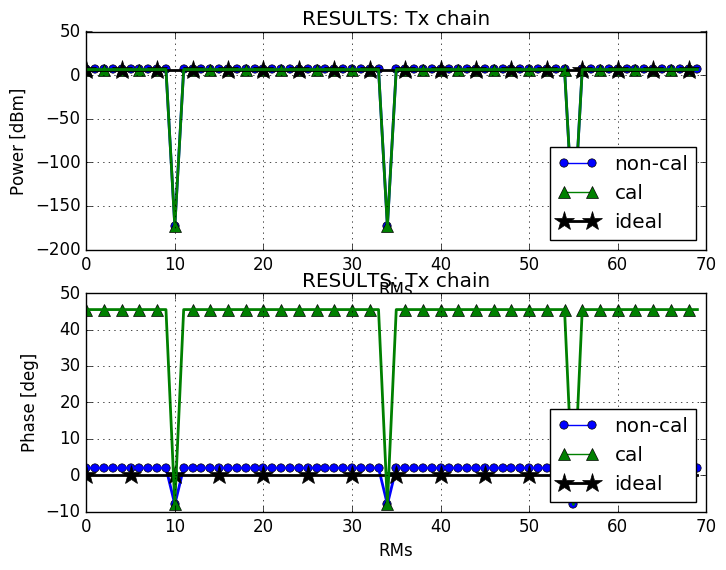
\includegraphics[width=10cm]{gfx/deadTRMsClassical0deg.png}}
 	
	\subfloat[]{
		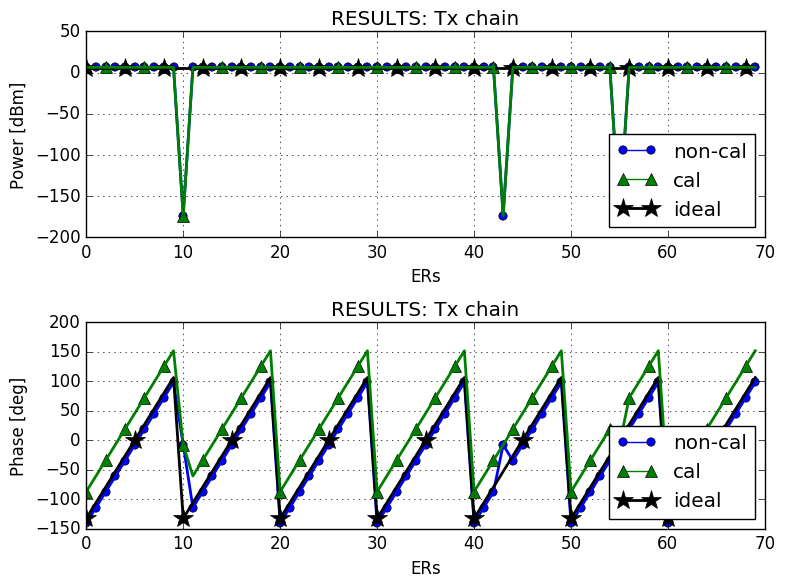
\includegraphics[width=8cm]{gfx/deadTRMsClassical10degCol.png}}
	\subfloat[]{
		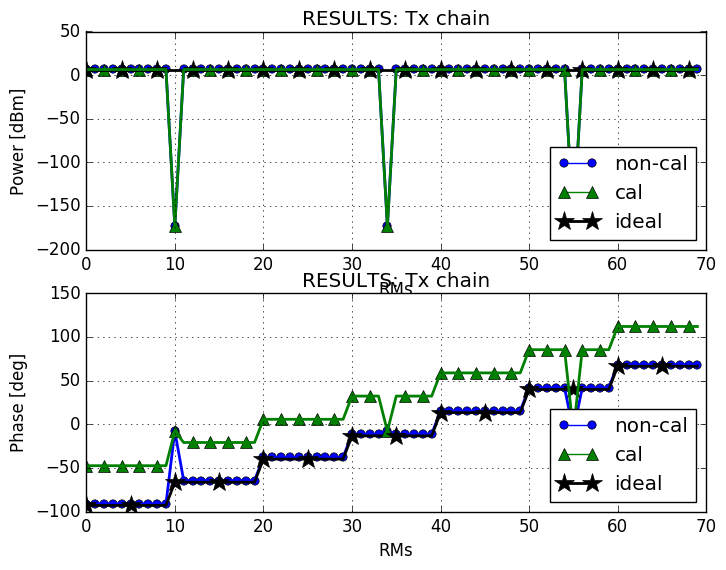
\includegraphics[width=8cm]{gfx/deadTRMsClassical10degRow.png}}
		\caption{Ganancia transmitida utilizando calibración clásica. (a) 0 grados. (b) 10 grados en 
		dirección horizontal. (c) 10 grados en dirección vertical.}
	\label{fig:deadTRMsClassical}
\end{figure}
En las figuras \ref{fig:deadTRMsClassicalPat} se observan los cortes de los patrones de antena horizontales y 
verticales. Si bien hay tres TRMs sin funcionar correctamente, se puede determinar que el patrón no se deforma 
significativamente. 
\begin{figure}[H]
	\centering
 	\subfloat[]{
		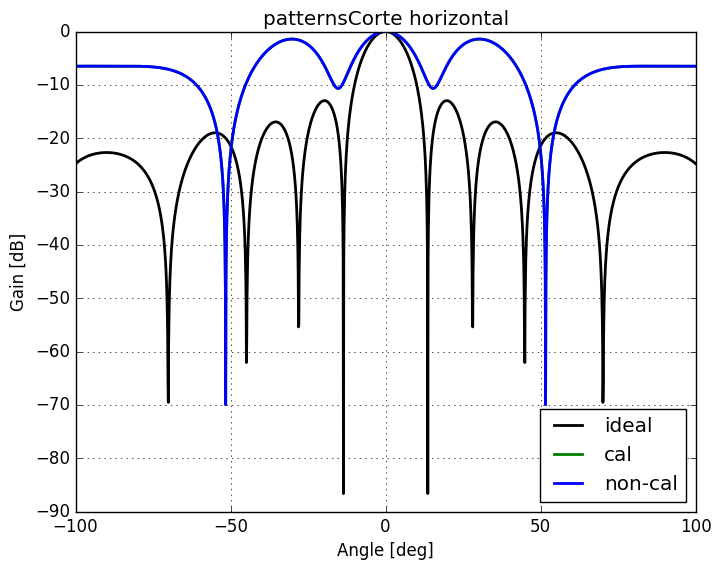
\includegraphics[width=8cm]{gfx/deadTRMsClassical0degAzCut.png}}
 	\subfloat[]{
		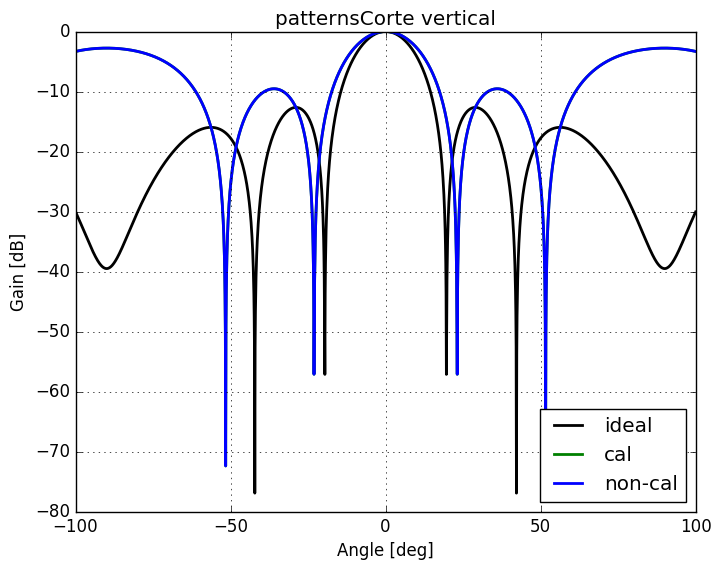
\includegraphics[width=8cm]{gfx/deadTRMsClassical0degElCut.png}}
 	
	\subfloat[]{
		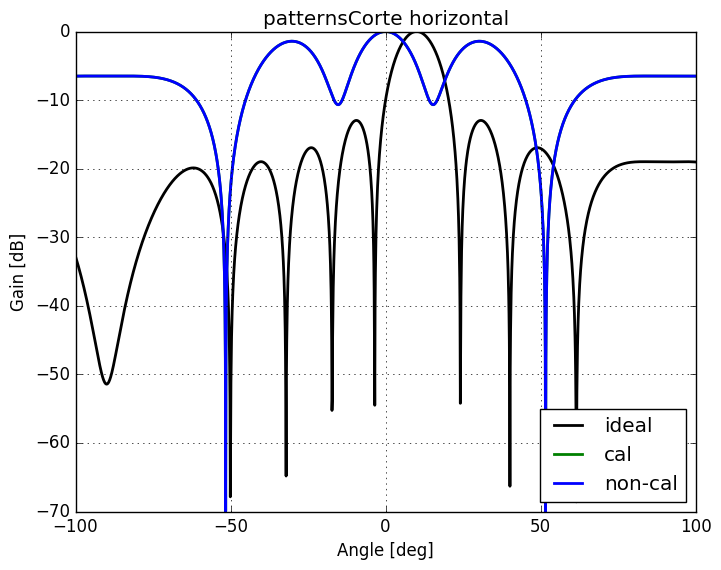
\includegraphics[width=8cm]{gfx/deadTRMsClassical10degColAzCut.png}}
	\subfloat[]{
		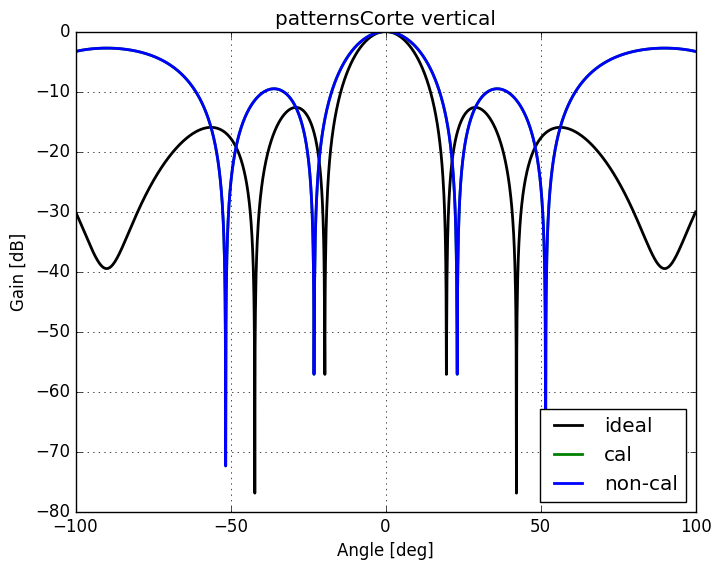
\includegraphics[width=8cm]{gfx/deadTRMsClassical10degColElCut.png}}

	\subfloat[]{
		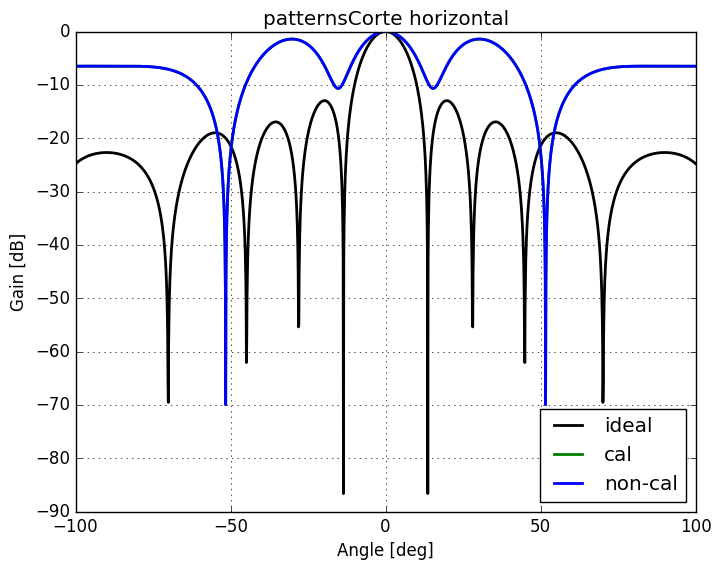
\includegraphics[width=8cm]{gfx/deadTRMsClassical10degRowAzCut.png}}
	\subfloat[]{
		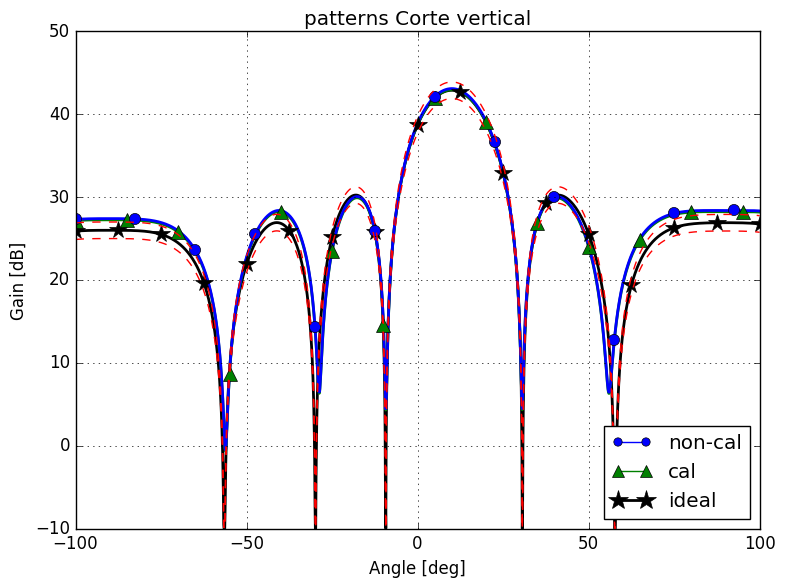
\includegraphics[width=8cm]{gfx/deadTRMsClassical10degRowElCut.png}}
		\caption{Patrones de antena transmitida utilizando calibración clásica. (a) uniforme - Corte Horizontal. (b) uniforme - 
			Corte Vertical. (c) 10 grados dir. horizontal. - Corte Horizontal. (d) 10 grados dir. horizontal. - Corte Vertical. (e) 10 
			grados dir. vertical - Corte Horizontal. (f) 10 grados dir. vertical - Corte Vertical.}
	\label{fig:deadTRMsClassicalPat}
\end{figure}

\begin{table}[H]
  \footnotesize
  \centering
  \begin{tabular}{|c|c|p{2cm}|p{2cm}|p{2cm}|p{2cm}|}
    \cline{2-6}
    \multicolumn{1}{c|}{} & \textbf{Corte} & \textbf{Potencia - lóbulo izquierdo} & \textbf{Potencia - lóbulo central} &
    \textbf{Potencia - lóbulo derecho} & \textbf{Ancho - lóbulo central} \tabularnewline\hline
    \multirow{2}{*}{\textbf{patrón sin calibrar}} & H & 27.6 & 38.89 & 27.08 & 12.0 \tabularnewline\cline{2-6}
     & V & 30.46 & 43.1 & 30.46 & 17.8 \tabularnewline\hline
    \multirow{2}{*}{\textbf{Patrón calibrada}} & H & 27.45 & 38.74 & 26.93 & 12.0 \tabularnewline\cline{2-6}
     & V & 30.31 & 42.96 & 30.31 & 17.8 \tabularnewline\hline
    \multirow{2}{*}{\textbf{Patrón ideal}} & H & 25.79 & 38.76 & 25.79 & 12.0 \tabularnewline\cline{2-6}
     & V & 30.25 & 42.9 & 30.25 & 17.8 \tabularnewline\hline
    \multirow{2}{*}{\textbf{Diferencia sin calibrar}} & H & 1.81 & 0.13 & 1.29 & 0.0\tabularnewline\cline{2-6}
     & V & 0.21 & 0.2 & 0.21 & 0.0 \tabularnewline\hline
    \multirow{2}{*}{\textbf{Diferencia calibrada}} & H & 1.66 & -0.02 & 1.14 & 0.0 \tabularnewline\cline{2-6}
     & V & 0.06 & 0.06 & 0.06 & 0.0 \tabularnewline\hline
  \end{tabular}
  \caption{Propiedades de los patrones calibrados y sin calibrar comparados con el ideal.}
  \label{tab:deadTRMsClassical10degRow}
\end{table}



\subsection{Utilizando la calibración con acoplamientos mútuos}

\subsubsection{Uniforme}

\subsubsection{Apuntamiento 10 grados en dirección horizontal}

\subsubsection{Apuntamiento 10 grados en dirección vertical}


En las figuras \ref{fig:deadTRMsMutual} se puede observar que independientemente de que se hayan destruído varios TRMs, el 
método puede calibrar los lazos, obteniendo los valores deseados, tanto de fase como de ganancia del resto de los elementos.
\begin{figure}[H]
	\centering
 	\subfloat[]{
		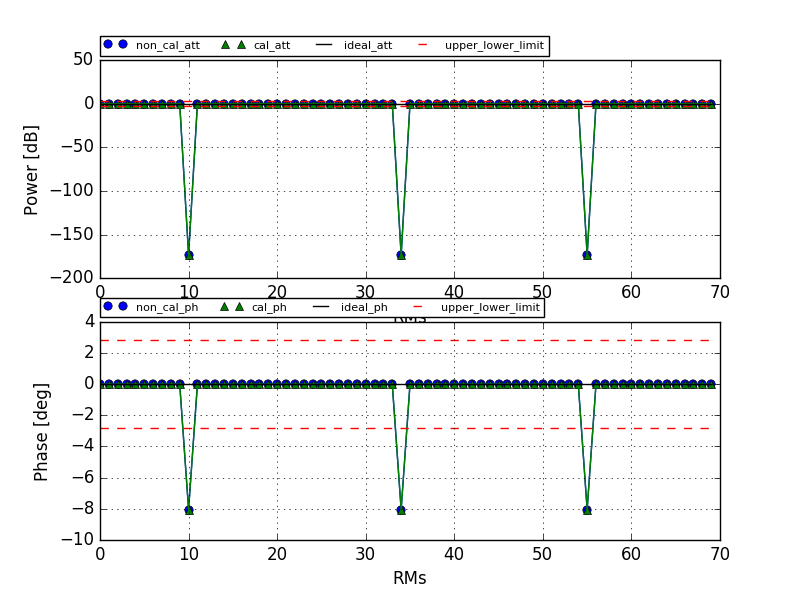
\includegraphics[width=10cm]{gfx/deadTRMsMutual0deg.png}}
 	
	\subfloat[]{
		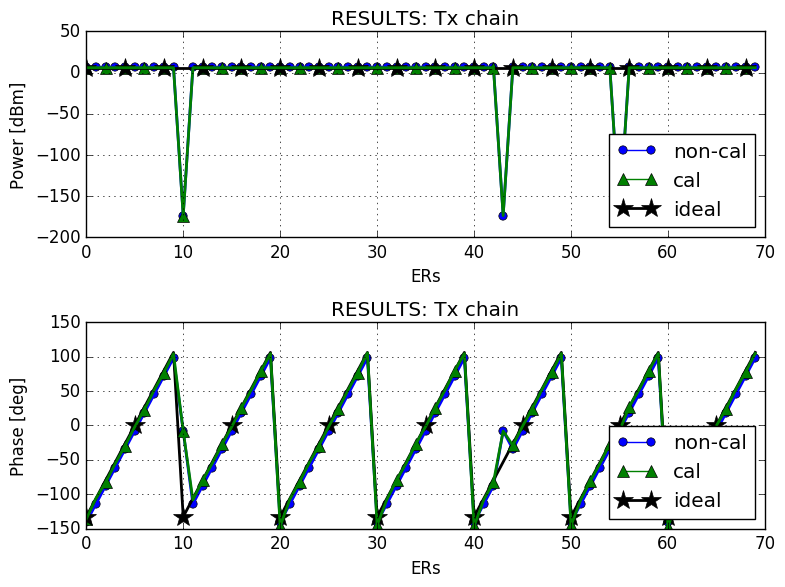
\includegraphics[width=8cm]{gfx/deadTRMsMutual10degCol.png}}
	\subfloat[]{
		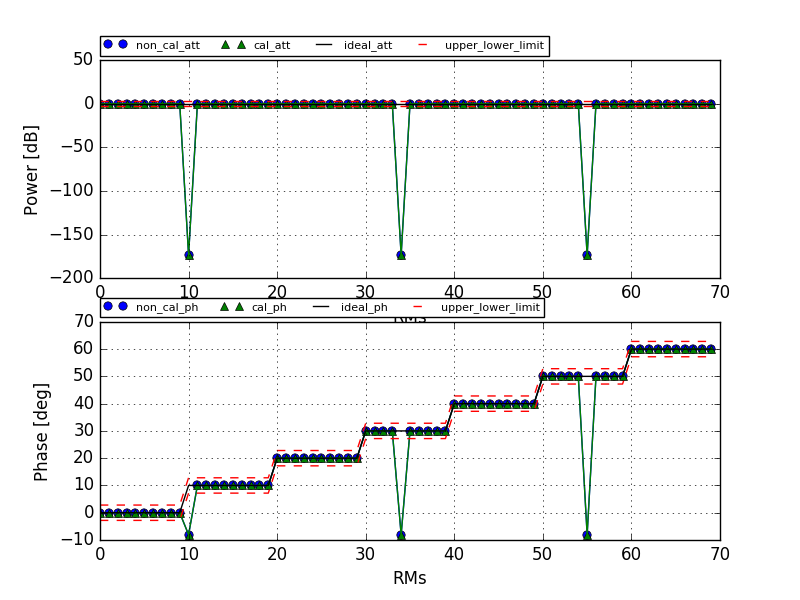
\includegraphics[width=8cm]{gfx/deadTRMsMutual10degRow.png}}
		\caption{Ganancia transmitida utilizando calibración con acoplamientos mútuos. (a) 0 grados. (b) 10 grados en 
		dirección horizontal. (c) 10 grados en dirección vertical.}
	\label{fig:deadTRMsMutual}
\end{figure}

\begin{figure}[H]
	\centering
 	\subfloat[]{
		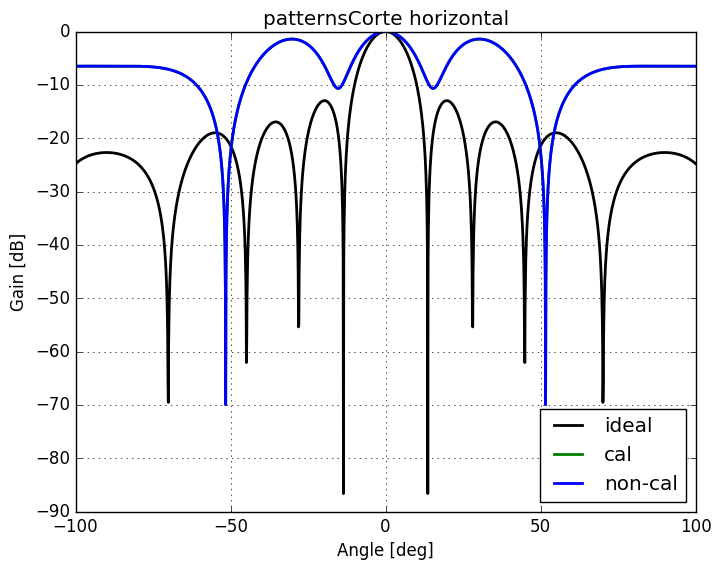
\includegraphics[width=8cm]{gfx/deadTRMsMutual0degAzCut.png}}
 	\subfloat[]{
		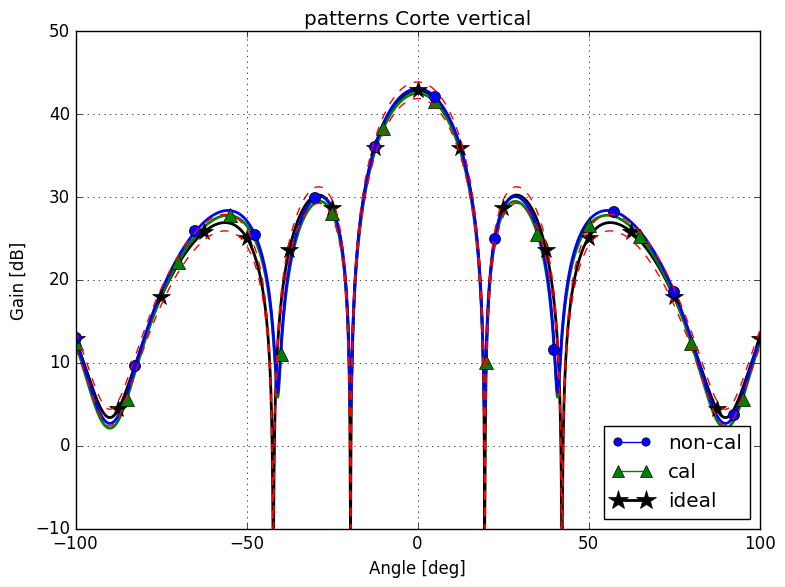
\includegraphics[width=8cm]{gfx/deadTRMsMutual0degElCut.png}}
 	
	\subfloat[]{
		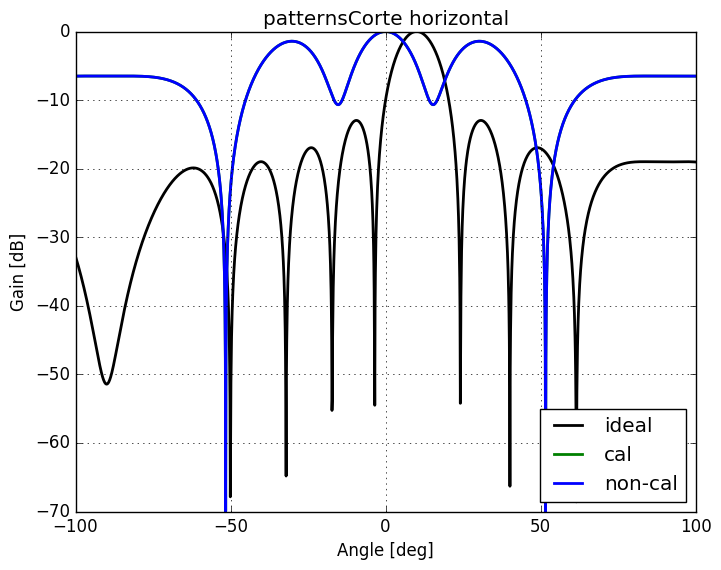
\includegraphics[width=8cm]{gfx/deadTRMsMutual10degColAzCut.png}}
	\subfloat[]{
		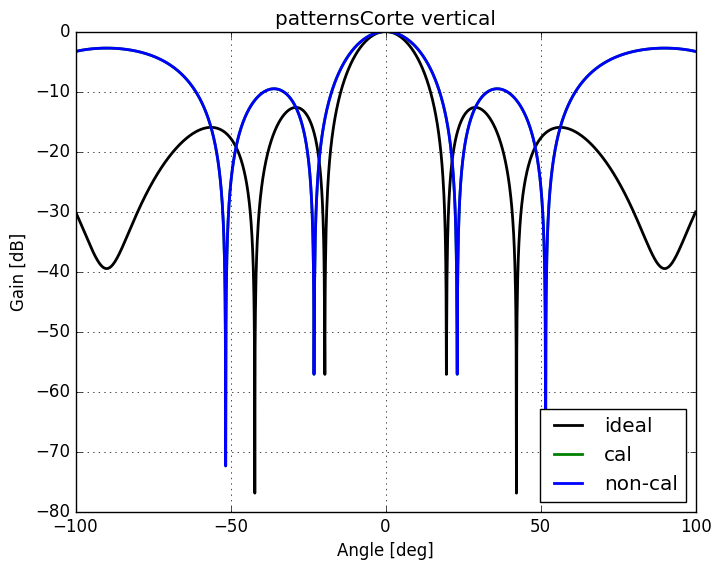
\includegraphics[width=8cm]{gfx/deadTRMsMutual10degColElCut.png}}

	\subfloat[]{
		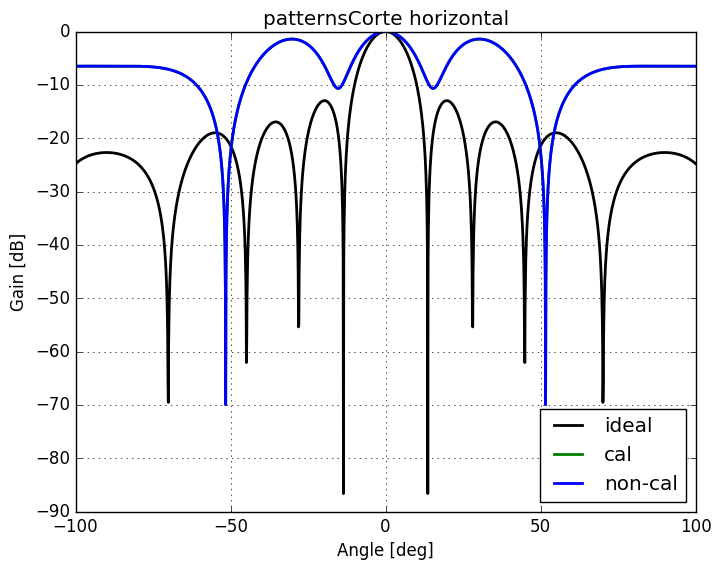
\includegraphics[width=8cm]{gfx/deadTRMsMutual10degRowAzCut.png}}
	\subfloat[]{
		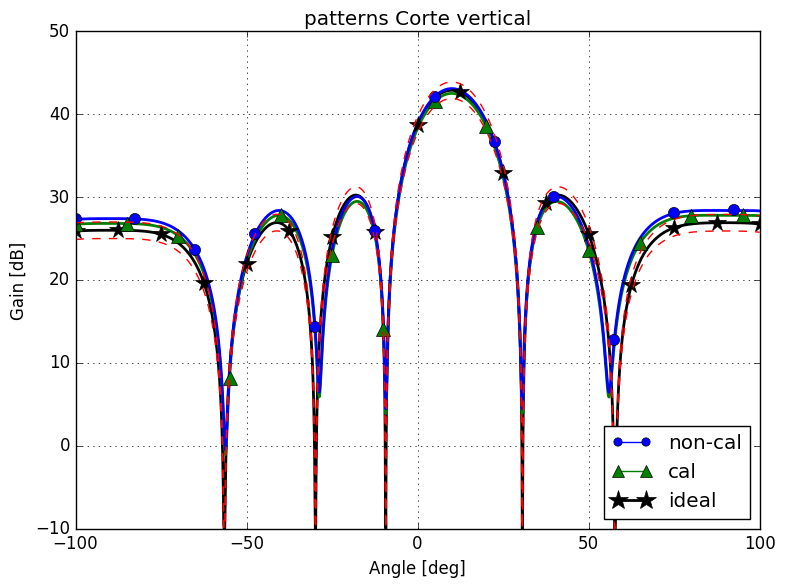
\includegraphics[width=8cm]{gfx/deadTRMsMutual10degRowElCut.png}}
		\caption{Patrones de antena transmitida utilizando calibración con acoplamientos mútuos. (a) uniforme - Corte Horizontal.
			(b) uniforme - Corte Vertical. (c) 10 grados dir. horizontal. - Corte Horizontal. (d) 10 grados dir. horizontal. - Corte 
			Vertical. (e) 10 grados dir. vertical - Corte Horizontal. (f) 10 grados dir. vertical - Corte Vertical.}
	\label{fig:deadTRMsMutualPat}
\end{figure}

\begin{table}[H]
  \footnotesize
  \centering
  \begin{tabular}{|c|c|p{2cm}|p{2cm}|p{2cm}|p{2cm}|}
    \cline{2-6}
    \multicolumn{1}{c|}{} & \textbf{Corte} & \textbf{Potencia - lóbulo izquierdo} & \textbf{Potencia - lóbulo central} &
    \textbf{Potencia - lóbulo derecho} & \textbf{Ancho - lóbulo central} \tabularnewline\hline
    \multirow{2}{*}{\textbf{patrón sin calibrar}} & H & 27.6 & 38.89 & 27.08 & 12.0 \tabularnewline\cline{2-6}
     & V & 30.46 & 43.1 & 30.46 & 17.8 \tabularnewline\hline
    \multirow{2}{*}{\textbf{Patrón calibrada}} & H & 27.02 & 38.31 & 26.5 & 12.0 \tabularnewline\cline{2-6}
     & V & 29.88 & 42.52 & 29.88 & 17.8 \tabularnewline\hline
    \multirow{2}{*}{\textbf{Patrón ideal}} & H & 25.79 & 38.76 & 25.79 & 12.0 \tabularnewline\cline{2-6}
     & V & 30.25 & 42.9 & 30.25 & 17.8 \tabularnewline\hline
    \multirow{2}{*}{\textbf{Diferencia sin calibrar}} & H & 1.81 & 0.13 & 1.29 & 0.0\tabularnewline\cline{2-6}
     & V & 0.21 & 0.2 & 0.21 & 0.0 \tabularnewline\hline
    \multirow{2}{*}{\textbf{Diferencia calibrada}} & H & 1.23 & -0.45 & 0.71 & 0.0 \tabularnewline\cline{2-6}
     & V & -0.37 & -0.38 & -0.37 & 0.0 \tabularnewline\hline
  \end{tabular}
  \caption{Propiedades de los patrones calibrados y sin calibrar comparados con el ideal.}
  \label{tab:deadTRMsMutual10degRow}
\end{table}


\section{Dispersiones en comportamiento de componentes de la antena}

Los ensayos de esta sección tienen las siguientes caracterísiticas,
\begin{itemize}
	\item Hay dispersiones de comportamiento en los siguientes componentes de la antena: circuladores, TRMs, PSCs y RMs. Las 
		magnitudes están especificadas en la tabla \ref{tab:errorReferences}.
		\begin{table}[H]
		  \footnotesize
		  \centering
		  \begin{tabular}{|c|c|}
			\hline
			\textbf{Error de componente} & \textbf{Desvío estandar} \tabularnewline \hline 
			Dispersión de ganancia del circulador &  0.2 [dB] \tabularnewline\hline 
			Dispersión de fase del circulador &  10 [deg] \tabularnewline\hline 
			Dispersión de ganancia del TRM &  0.2 [dB] \tabularnewline\hline 
			Dispersión de fase del TRM &  10 [deg] \tabularnewline\hline 
			Dispersión de ganancia del PSC &  0.1 [dB] \tabularnewline\hline 
			Dispersión de fase del PSC &  10 [deg] \tabularnewline\hline 
		  \end{tabular}
		  \caption{Configuración de los errores de componentes.}
		  \label{tab:errorReferences}
		\end{table}
	\item No hay errores de calibración.
	\item No hay errores en la señal.
\end{itemize}

\subsection{Utilizando la calibración clásica}

\subsubsection{Uniforme}

\subsubsection{Apuntamiento 10 grados en dirección horizontal}

\subsubsection{Apuntamiento 10 grados en dirección vertical}


\begin{figure}[H]
	\centering
 	\subfloat[]{
		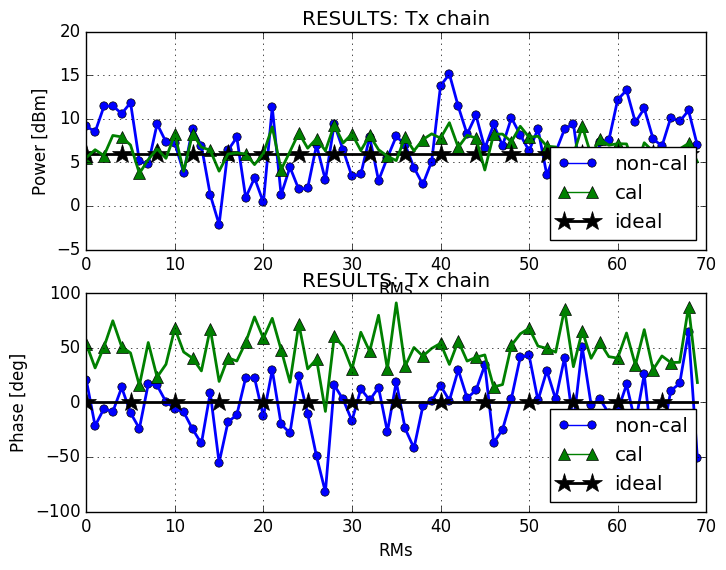
\includegraphics[width=10cm]{gfx/compErrClassical0deg.png}}
 	
	\subfloat[]{
		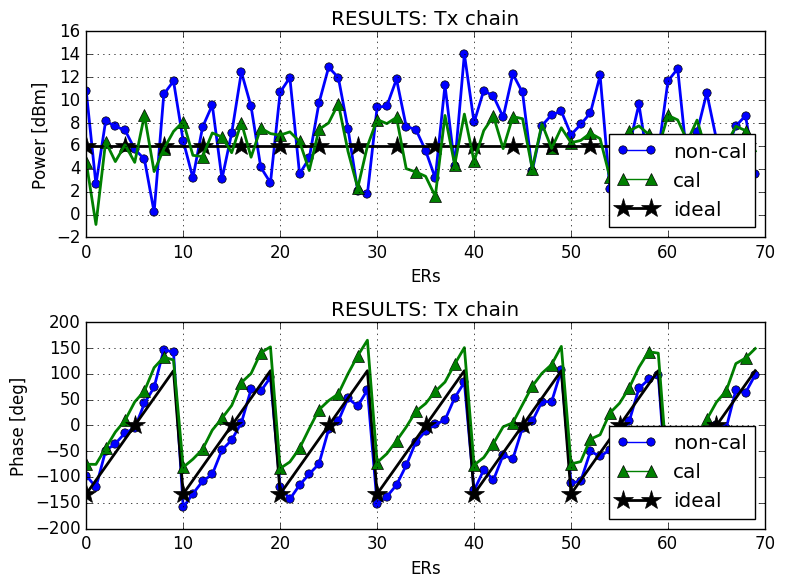
\includegraphics[width=8cm]{gfx/compErrClassical10degCol.png}}
	\subfloat[]{
		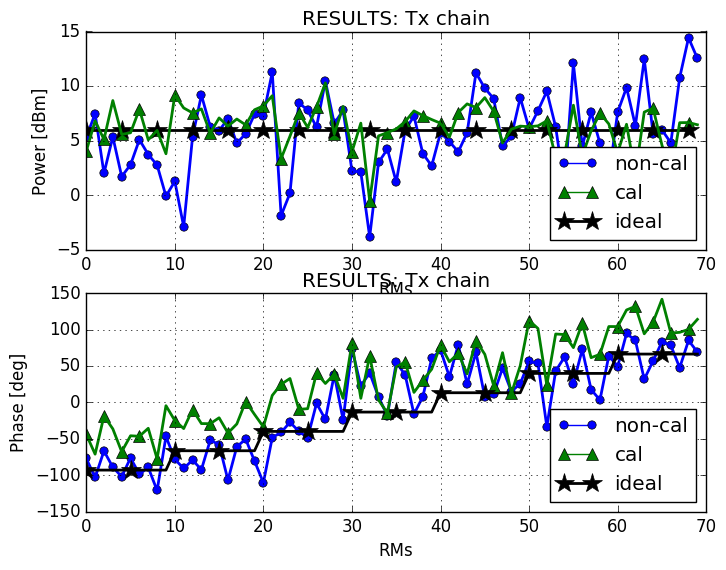
\includegraphics[width=8cm]{gfx/compErrClassical10degRow.png}}
		\caption{Ganancia transmitida utilizando calibración clásica. (a) 0 grados. (b) 10 grados en 
		dirección horizontal. (c) 10 grados en dirección vertical.}
	\label{fig:compErrClassical}
\end{figure}
\begin{figure}[H]
	\centering
 	\subfloat[]{
		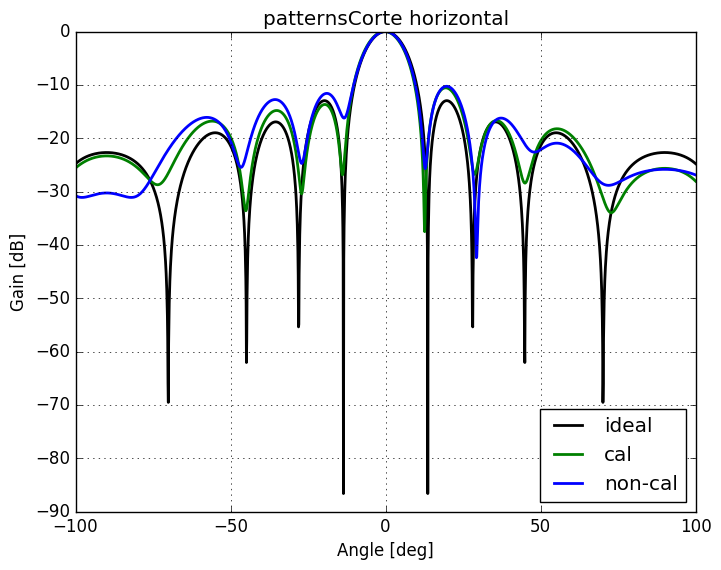
\includegraphics[width=8cm]{gfx/compErrClassical0degAzCut.png}}
 	\subfloat[]{
		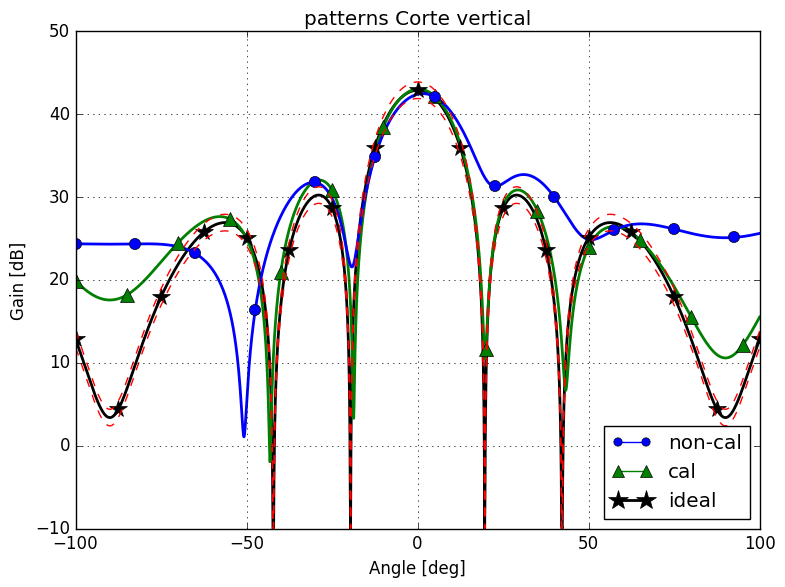
\includegraphics[width=8cm]{gfx/compErrClassical0degElCut.png}}
 	
	\subfloat[]{
		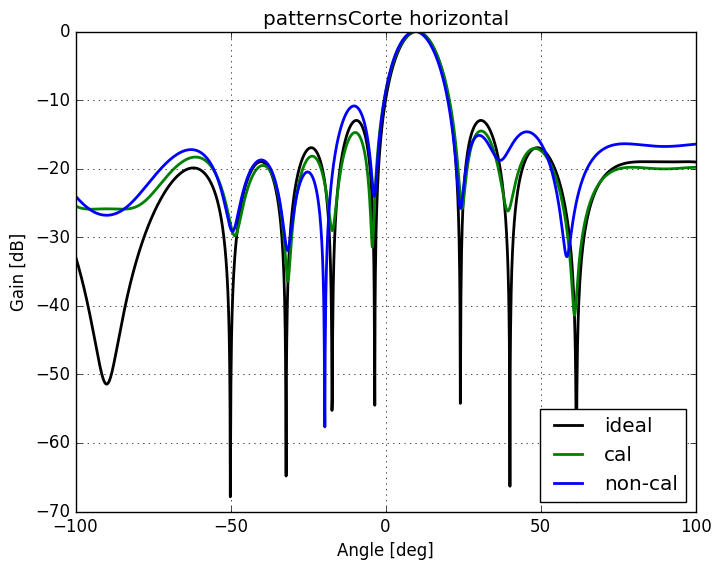
\includegraphics[width=8cm]{gfx/compErrClassical10degColAzCut.png}}
	\subfloat[]{
		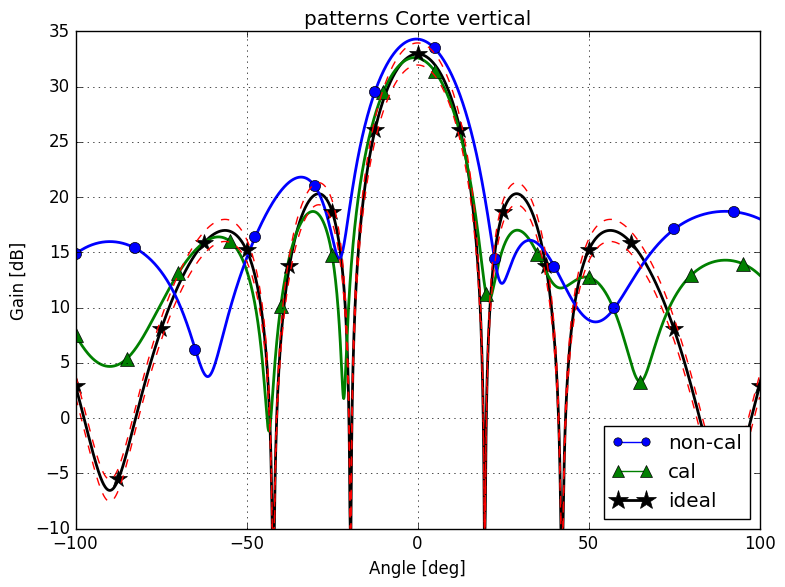
\includegraphics[width=8cm]{gfx/compErrClassical10degColElCut.png}}

	\subfloat[]{
		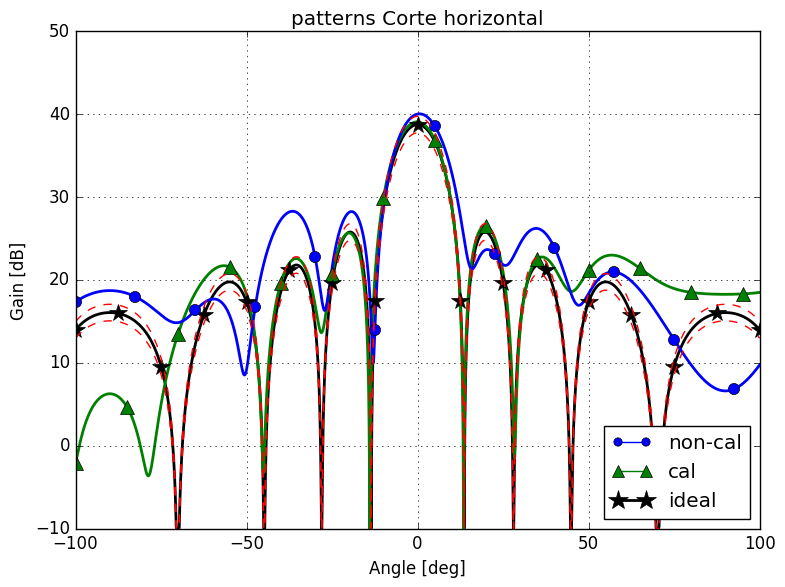
\includegraphics[width=8cm]{gfx/compErrClassical10degRowAzCut.png}}
	\subfloat[]{
		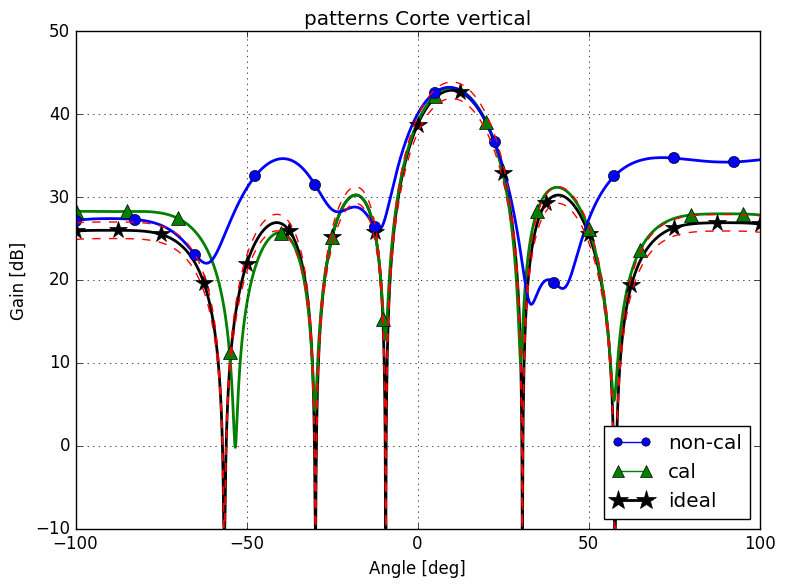
\includegraphics[width=8cm]{gfx/compErrClassical10degRowElCut.png}}
		\caption{Patrones de antena transmitida utilizando calibración clásica. (a) uniforme - Corte Horizontal. (b) uniforme - 
			Corte Vertical. (c) 10 grados dir. horizontal. - Corte Horizontal. (d) 10 grados dir. horizontal. - Corte Vertical. (e) 10 
			grados dir. vertical - Corte Horizontal. (f) 10 grados dir. vertical - Corte Vertical.}
	\label{fig:compErrClassicalPat}
\end{figure}

\begin{table}[H]
  \footnotesize
  \centering
  \begin{tabular}{|c|c|p{2cm}|p{2cm}|p{2cm}|p{2cm}|}
    \cline{2-6}
    \multicolumn{1}{c|}{} & \textbf{Corte} & \textbf{Potencia - lóbulo izquierdo} & \textbf{Potencia - lóbulo central} &
    \textbf{Potencia - lóbulo derecho} & \textbf{Ancho - lóbulo central} \tabularnewline\hline
    \multirow{2}{*}{\textbf{patrón sin calibrar}} & H & 27.09 & 38.77 & 29.26 & 11.4 \tabularnewline\cline{2-6}
     & V & 32.95 & 41.49 & 32.59 & 16.8 \tabularnewline\hline
    \multirow{2}{*}{\textbf{Patrón calibrada}} & H & 26.62 & 38.88 & 27.41 & 12.0 \tabularnewline\cline{2-6}
     & V & 32.18 & 42.72 & 28.34 & 18.0 \tabularnewline\hline
    \multirow{2}{*}{\textbf{Patrón ideal}} & H & 25.79 & 38.76 & 25.79 & 12.0 \tabularnewline\cline{2-6}
     & V & 30.25 & 42.9 & 30.25 & 17.8 \tabularnewline\hline
    \multirow{2}{*}{\textbf{Diferencia sin calibrar}} & H & 1.3 & 0.01 & 3.47 & -0.6\tabularnewline\cline{2-6}
     & V & 2.7 & -1.41 & 2.34 & -1.0 \tabularnewline\hline
    \multirow{2}{*}{\textbf{Diferencia calibrada}} & H & 0.83 & 0.12 & 1.62 & 0.0 \tabularnewline\cline{2-6}
     & V & 1.93 & -0.18 & -1.91 & 0.2 \tabularnewline\hline
  \end{tabular}
  \caption{Propiedades de los patrones calibrados y sin calibrar comparados con el ideal.}
  \label{tab:compErrClassical10degRow}
\end{table}


\subsection{Utilizando la calibración con acoplamientos mútuos}

\subsubsection{Uniforme}

\subsubsection{Apuntamiento 10 grados en dirección horizontal}

\subsubsection{Apuntamiento 10 grados en dirección vertical}


En la figura \ref{fig:compErrMutual} se puede observar que si bien, en algunos ensayos el método no corrige 
perfectamente la fase por el error agregado de todos los componentes de la RFDN a la vez, en una segunda iteración se logra 
llegar a dicho valor. La subfigura (a) muestra un apuntamiento de cero grados, la (b), de 10 grados en 
dirección horizontal, y la tercera de 10 grados en dirección vertical.
\begin{figure}[H]
	\centering
 	\subfloat[]{
		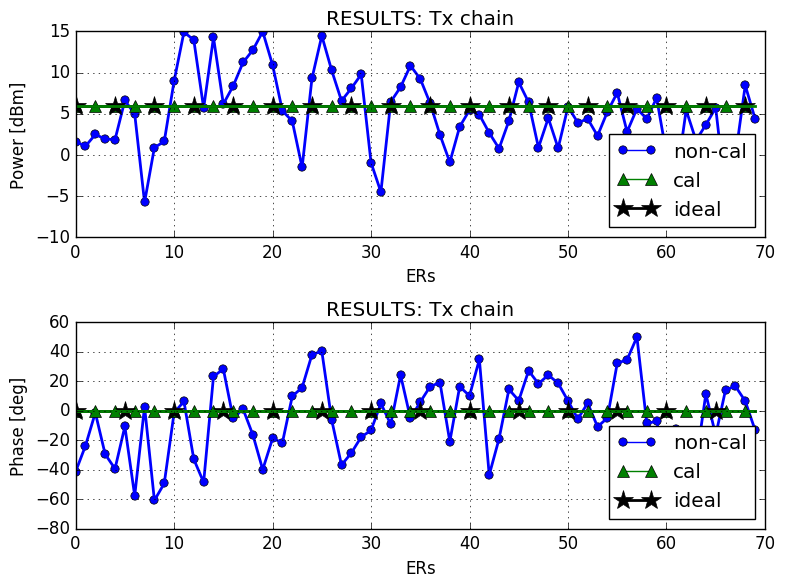
\includegraphics[width=10cm]{gfx/compErrMutual0deg.png}}
 	
	\subfloat[]{
		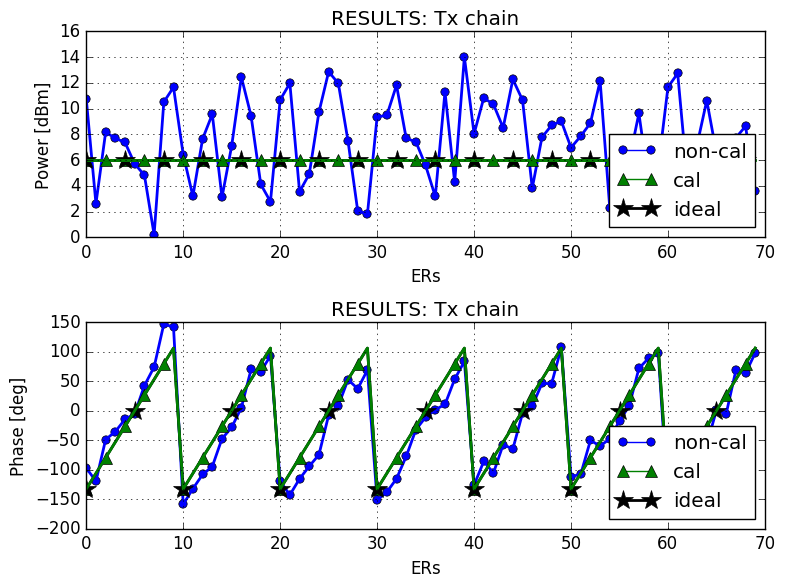
\includegraphics[width=8cm]{gfx/compErrMutual10degCol.png}}
	\subfloat[]{
		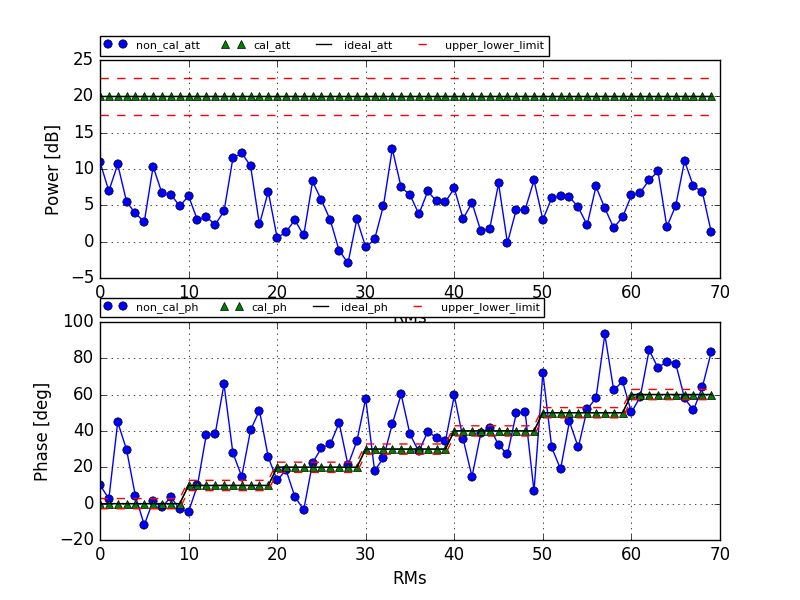
\includegraphics[width=8cm]{gfx/compErrMutual10degRow.png}}
		\caption{Ganancia transmitida utilizando calibración con acoplamientos mútuos. (a) 0 grados. (b) 10 grados en 
		dirección horizontal. (c) 10 grados en dirección vertical.}
	\label{fig:compErrMutual}
\end{figure}
\begin{figure}[H]
	\centering
 	\subfloat[]{
		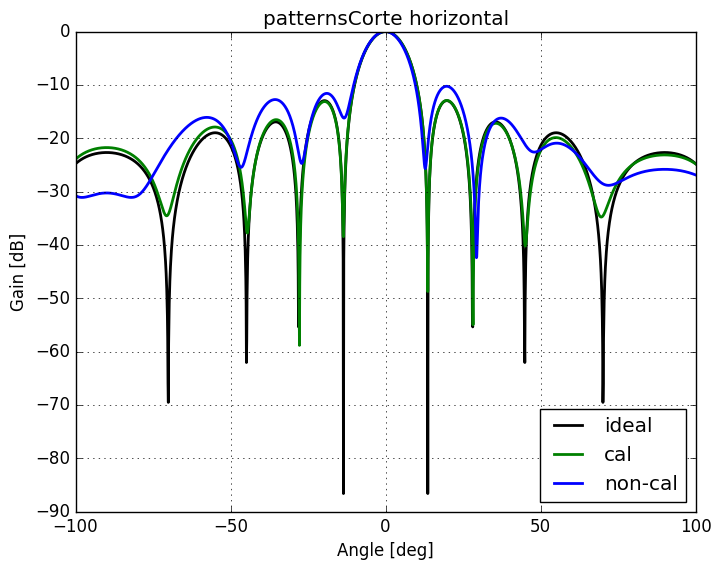
\includegraphics[width=8cm]{gfx/compErrMutual0degAzCut.png}}
 	\subfloat[]{
		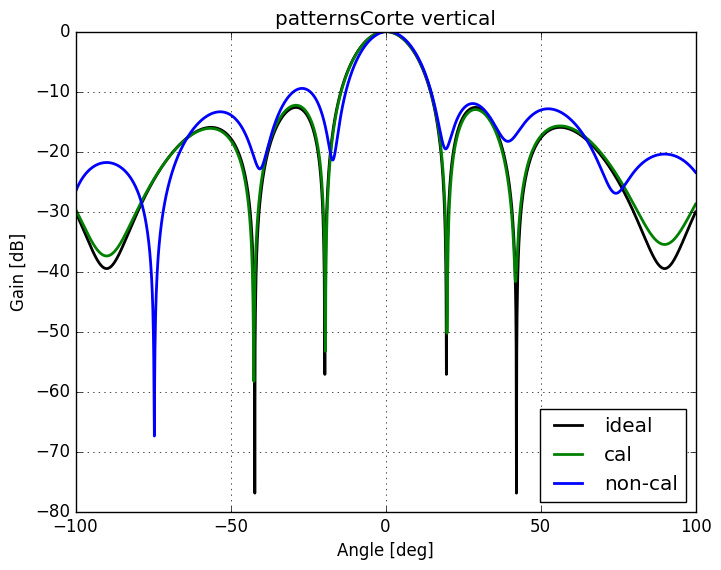
\includegraphics[width=8cm]{gfx/compErrMutual0degElCut.png}}
 	
	\subfloat[]{
		\includegraphics[width=8cm]{gfx/compErrMutual10degColAzCut.png}}
	\subfloat[]{
		\includegraphics[width=8cm]{gfx/compErrMutual10degColElCut.png}}

	\subfloat[]{
		\includegraphics[width=8cm]{gfx/compErrMutual10degRowAzCut.png}}
	\subfloat[]{
		\includegraphics[width=8cm]{gfx/compErrMutual10degRowElCut.png}}
		\caption{Patrones de antena transmitida utilizando calibración con acoplamientos mútuos. (a) uniforme - Corte Horizontal.
			(b) uniforme - Corte Vertical. (c) 10 grados dir. horizontal. - Corte Horizontal. (d) 10 grados dir. horizontal. - Corte 
			Vertical. (e) 10 grados dir. vertical - Corte Horizontal. (f) 10 grados dir. vertical - Corte Vertical.}
	\label{fig:compErrMutualPat}
\end{figure}

\begin{table}[H]
  \footnotesize
  \centering
  \begin{tabular}{|c|c|p{2cm}|p{2cm}|p{2cm}|p{2cm}|}
    \cline{2-6}
    \multicolumn{1}{c|}{} & \textbf{Corte} & \textbf{Potencia del lóbulo secundario izquierdo} & \textbf{Potencia del lóbulo principal} &
    \textbf{Potencia del lóbulo secundario derecho} & \textbf{Ancho del lóbulo principal} \tabularnewline\hline
    \multirow{2}{*}{\textbf{patrón sin calibrar}} & H & 26.37 & 39.34 & 26.37 & 12.0 \tabularnewline\cline{2-6}
     & V & 30.83 & 43.48 & 30.83 & 17.8 \tabularnewline\hline
    \multirow{2}{*}{\textbf{Patrón calibrada}} & H & 25.79 & 38.76 & 25.79 & 12.0 \tabularnewline\cline{2-6}
     & V & 30.25 & 42.9 & 30.25 & 17.8 \tabularnewline\hline
    \multirow{2}{*}{\textbf{Patrón ideal}} & H & 25.79 & 38.76 & 25.79 & 12.0 \tabularnewline\cline{2-6}
     & V & 30.25 & 42.9 & 30.25 & 17.8 \tabularnewline\hline
    \multirow{2}{*}{\textbf{Diferencia sin calibrar}} & H & 0.58 & 0.58 & 0.58 & 0.0\tabularnewline\cline{2-6}
     & V & 0.58 & 0.58 & 0.58 & 0.0 \tabularnewline\hline
    \multirow{2}{*}{\textbf{Diferencia calibrada}} & H & 0.0 & 0.0 & 0.0 & 0.0 \tabularnewline\cline{2-6}
     & V & 0.0 & 0.0 & 0.0 & 0.0 \tabularnewline\hline
  \end{tabular}
  \caption{Propiedades de los patrones calibrados y sin calibrar comparados con el ideal.}
  \label{tab:comErrMutual10degRow}
\end{table}


\section{Dispersiones de ganancia entre pulsos}

\subsection{Utilizando la calibración clásica}

\subsubsection{Uniforme}

\subsubsection{Apuntamiento 10 grados en dirección horizontal}

\subsubsection{Apuntamiento 10 grados en dirección vertical}


\begin{figure}[H]
	\centering
 	\subfloat[]{
		\includegraphics[width=10cm]{gfx/chirpErrClassical0deg.png}}
 	
	\subfloat[]{
		\includegraphics[width=8cm]{gfx/chirpErrClassical10degCol.png}}
	\subfloat[]{
		\includegraphics[width=8cm]{gfx/chirpErrClassical10degRow.png}}
		\caption{Ganancia transmitida utilizando calibración clásica. (a) 0 grados. (b) 10 grados en 
		dirección horizontal. (c) 10 grados en dirección vertical.}
	\label{fig:chirpErrClassical}
\end{figure}
\begin{figure}[H]
	\centering
 	\subfloat[]{
		\includegraphics[width=8cm]{gfx/chirpErrClassical0degAzCut.png}}
 	\subfloat[]{
		\includegraphics[width=8cm]{gfx/chirpErrClassical0degElCut.png}}
 	
	\subfloat[]{
		\includegraphics[width=8cm]{gfx/chirpErrClassical10degColAzCut.png}}
	\subfloat[]{
		\includegraphics[width=8cm]{gfx/chirpErrClassical10degColElCut.png}}

	\subfloat[]{
		\includegraphics[width=8cm]{gfx/chirpErrClassical10degRowAzCut.png}}
	\subfloat[]{
		\includegraphics[width=8cm]{gfx/chirpErrClassical10degRowElCut.png}}
		\caption{Patrones de antena transmitida utilizando calibración clásica. (a) uniforme - Corte Horizontal. (b) uniforme - 
			Corte Vertical. (c) 10 grados dir. horizontal. - Corte Horizontal. (d) 10 grados dir. horizontal. - Corte Vertical. (e) 10 
			grados dir. vertical - Corte Horizontal. (f) 10 grados dir. vertical - Corte Vertical.}
	\label{fig:chirpErrClassicalPat}
\end{figure}

\begin{table}[H]
  \footnotesize
  \centering
  \begin{tabular}{|c|c|p{2cm}|p{2cm}|p{2cm}|p{2cm}|}
    \cline{2-6}
    \multicolumn{1}{c|}{} & \textbf{Corte} & \textbf{Potencia - lóbulo izquierdo} & \textbf{Potencia - lóbulo central} &
    \textbf{Potencia - lóbulo derecho} & \textbf{Ancho - lóbulo central} \tabularnewline\hline
    \multirow{2}{*}{\textbf{patrón sin calibrar}} & H & 26.37 & 39.34 & 26.37 & 12.0 \tabularnewline\cline{2-6}
     & V & 30.83 & 43.48 & 30.83 & 17.8 \tabularnewline\hline
    \multirow{2}{*}{\textbf{Patrón calibrada}} & H & 15.15 & 23.47 & 14.44 & 11.8 \tabularnewline\cline{2-6}
     & V & 25.82 & 38.8 & 0 & 27.6 \tabularnewline\hline
    \multirow{2}{*}{\textbf{Patrón ideal}} & H & 25.79 & 38.76 & 25.79 & 12.0 \tabularnewline\cline{2-6}
     & V & 30.25 & 42.9 & 30.25 & 17.8 \tabularnewline\hline
    \multirow{2}{*}{\textbf{Diferencia sin calibrar}} & H & 0.58 & 0.58 & 0.58 & 0.0\tabularnewline\cline{2-6}
     & V & 0.58 & 0.58 & 0.58 & 0.0 \tabularnewline\hline
    \multirow{2}{*}{\textbf{Diferencia calibrada}} & H & -10.64 & -15.29 & -11.35 & -0.2 \tabularnewline\cline{2-6}
     & V & -4.43 & -4.1 & -30.25 & 9.8 \tabularnewline\hline
  \end{tabular}
  \caption{Propiedades de los patrones calibrados y sin calibrar comparados con el ideal.}
  \label{tab:chirpErrClassical10degRow}
\end{table}


\subsection{Utilizando la calibración con acoplamientos mútuos}

\subsubsection{Uniforme}

\subsubsection{Apuntamiento 10 grados en dirección horizontal}

\subsubsection{Apuntamiento 10 grados en dirección vertical}


\begin{figure}[H]
	\centering
 	\subfloat[]{
		\includegraphics[width=10cm]{gfx/chirpErrMutual0deg.png}}
 	
	\subfloat[]{
		\includegraphics[width=8cm]{gfx/chirpErrMutual10degCol.png}}
	\subfloat[]{
		\includegraphics[width=8cm]{gfx/chirpErrMutual10degRow.png}}
		\caption{Ganancia transmitida utilizando calibración con acoplamientos mútuos. (a) 0 grados. (b) 10 grados en 
		dirección horizontal. (c) 10 grados en dirección vertical.}
	\label{fig:chirpErrMutual}
\end{figure}
\begin{figure}[H]
	\centering
 	\subfloat[]{
		\includegraphics[width=8cm]{gfx/chirpErrMutual0degAzCut.png}}
 	\subfloat[]{
		\includegraphics[width=8cm]{gfx/chirpErrMutual0degElCut.png}}
 	
	\subfloat[]{
		\includegraphics[width=8cm]{gfx/chirpErrMutual10degColAzCut.png}}
	\subfloat[]{
		\includegraphics[width=8cm]{gfx/chirpErrMutual10degColElCut.png}}

	\subfloat[]{
		\includegraphics[width=8cm]{gfx/chirpErrMutual10degRowAzCut.png}}
	\subfloat[]{
		\includegraphics[width=8cm]{gfx/chirpErrMutual10degRowElCut.png}}
		\caption{Patrones de antena transmitida utilizando calibración con acoplamientos mútuos. (a) uniforme - Corte Horizontal.
			(b) uniforme - Corte Vertical. (c) 10 grados dir. horizontal. - Corte Horizontal. (d) 10 grados dir. horizontal. - Corte 
			Vertical. (e) 10 grados dir. vertical - Corte Horizontal. (f) 10 grados dir. vertical - Corte Vertical.}
	\label{fig:chirpErrMutualPat}
\end{figure}

\begin{table}[H]
  \footnotesize
  \centering
  \begin{tabular}{|c|c|p{2cm}|p{2cm}|p{2cm}|p{2cm}|}
    \cline{2-6}
    \multicolumn{1}{c|}{} & \textbf{Corte} & \textbf{Potencia - lóbulo izquierdo} & \textbf{Potencia - lóbulo central} &
    \textbf{Potencia - lóbulo derecho} & \textbf{Ancho - lóbulo central} \tabularnewline\hline
    \multirow{2}{*}{\textbf{patrón sin calibrar}} & H & 26.37 & 39.34 & 26.37 & 12.0 \tabularnewline\cline{2-6}
     & V & 30.83 & 43.48 & 30.83 & 17.8 \tabularnewline\hline
    \multirow{2}{*}{\textbf{Patrón calibrada}} & H & 25.79 & 38.76 & 25.79 & 12.0 \tabularnewline\cline{2-6}
     & V & 30.25 & 42.9 & 30.25 & 17.8 \tabularnewline\hline
    \multirow{2}{*}{\textbf{Patrón ideal}} & H & 25.79 & 38.76 & 25.79 & 12.0 \tabularnewline\cline{2-6}
     & V & 30.25 & 42.9 & 30.25 & 17.8 \tabularnewline\hline
    \multirow{2}{*}{\textbf{Diferencia sin calibrar}} & H & 0.58 & 0.58 & 0.58 & 0.0\tabularnewline\cline{2-6}
     & V & 0.58 & 0.58 & 0.58 & 0.0 \tabularnewline\hline
    \multirow{2}{*}{\textbf{Diferencia calibrada}} & H & 0.0 & 0.0 & 0.0 & 0.0 \tabularnewline\cline{2-6}
     & V & 0.0 & 0.0 & 0.0 & 0.0 \tabularnewline\hline
  \end{tabular}
  \caption{Propiedades de los patrones calibrados y sin calibrar comparados con el ideal.}
  \label{tab:chirpErrMutual10degRow}
\end{table}


\section{Dispersión de ganancia de la chirp réplica}

Como la chirp réplica es simplemente utilizada en la calibración clásica, en esta simulación no se podrán comparar 
resultados, pero sirve para determinar que tan robusto es el método para esta clase de erorres.
\begin{figure}[H]
	\centering
 	\subfloat[]{
		\includegraphics[width=10cm]{gfx/chirpRepErrClassical0deg.png}}
 	
	\subfloat[]{
		\includegraphics[width=8cm]{gfx/chirpRepErrClassical10degCol.png}}
	\subfloat[]{
		\includegraphics[width=8cm]{gfx/chirpRepErrClassical10degRow.png}}
		\caption{Ganancia transmitida utilizando calibración clásica. (a) 0 grados. (b) 10 grados en 
		dirección horizontal. (c) 10 grados en dirección vertical.}
	\label{fig:chirpRepErrClassical}
\end{figure}
\begin{figure}[H]
	\centering
 	\subfloat[]{
		\includegraphics[width=8cm]{gfx/chirpRepErrClassical0degAzCut.png}}
 	\subfloat[]{
		\includegraphics[width=8cm]{gfx/chirpRepErrClassical0degElCut.png}}
 	
	\subfloat[]{
		\includegraphics[width=8cm]{gfx/chirpRepErrClassical10degColAzCut.png}}
	\subfloat[]{
		\includegraphics[width=8cm]{gfx/chirpRepErrClassical10degColElCut.png}}

	\subfloat[]{
		\includegraphics[width=8cm]{gfx/chirpRepErrClassical10degRowAzCut.png}}
	\subfloat[]{
		\includegraphics[width=8cm]{gfx/chirpRepErrClassical10degRowElCut.png}}
		\caption{Patrones de antena transmitida utilizando calibración clásica. (a) uniforme - Corte Horizontal. (b) uniforme - 
			Corte Vertical. (c) 10 grados dir. horizontal. - Corte Horizontal. (d) 10 grados dir. horizontal. - Corte Vertical. (e) 10 
			grados dir. vertical - Corte Horizontal. (f) 10 grados dir. vertical - Corte Vertical.}
	\label{fig:chirpRepErrClassicalPat}
\end{figure}

\begin{table}[H]
  \footnotesize
  \centering
  \begin{tabular}{|c|c|p{2cm}|p{2cm}|p{2cm}|p{2cm}|}
    \cline{2-6}
    \multicolumn{1}{c|}{} & \textbf{Corte} & \textbf{Potencia - lóbulo izquierdo} & \textbf{Potencia - lóbulo central} &
    \textbf{Potencia - lóbulo derecho} & \textbf{Ancho - lóbulo central} \tabularnewline\hline
    \multirow{2}{*}{\textbf{patrón sin calibrar}} & H & 26.37 & 39.34 & 26.37 & 12.0 \tabularnewline\cline{2-6}
     & V & 30.83 & 43.48 & 30.83 & 17.8 \tabularnewline\hline
    \multirow{2}{*}{\textbf{Patrón calibrada}} & H & 19.69 & 32.65 & 19.69 & 12.0 \tabularnewline\cline{2-6}
     & V & 24.15 & 36.8 & 24.15 & 17.8 \tabularnewline\hline
    \multirow{2}{*}{\textbf{Patrón ideal}} & H & 25.79 & 38.76 & 25.79 & 12.0 \tabularnewline\cline{2-6}
     & V & 30.25 & 42.9 & 30.25 & 17.8 \tabularnewline\hline
    \multirow{2}{*}{\textbf{Diferencia sin calibrar}} & H & 0.58 & 0.58 & 0.58 & 0.0\tabularnewline\cline{2-6}
     & V & 0.58 & 0.58 & 0.58 & 0.0 \tabularnewline\hline
    \multirow{2}{*}{\textbf{Diferencia calibrada}} & H & -6.1 & -6.11 & -6.1 & 0.0 \tabularnewline\cline{2-6}
     & V & -6.1 & -6.1 & -6.1 & 0.0 \tabularnewline\hline
  \end{tabular}
  \caption{Propiedades de los patrones calibrados y sin calibrar comparados con el ideal.}
  \label{tab:chirpRepErrClassical10degRow}
\end{table}


\section{Dispersión de fase del Walsh}

Como los códigos walsh son solamente utilizados en la calibración clásica, en esta simulación no se podrán comparar 
resultados, pero sirve para determinar que tan robusto es el método para esta clase de erorres.
\begin{figure}[H]
	\centering
 	\subfloat[]{
		\includegraphics[width=10cm]{gfx/wallErrClassical0deg.png}}
 	
	\subfloat[]{
		\includegraphics[width=8cm]{gfx/wallErrClassical10degCol.png}}
	\subfloat[]{
		\includegraphics[width=8cm]{gfx/wallErrClassical10degRow.png}}
		\caption{Ganancia transmitida utilizando calibración clásica. (a) 0 grados. (b) 10 grados en 
		dirección horizontal. (c) 10 grados en dirección vertical.}
	\label{fig:wallErrClassical}
\end{figure}
\begin{figure}[H]
	\centering
 	\subfloat[]{
		\includegraphics[width=8cm]{gfx/wallErrClassical0degAzCut.png}}
 	\subfloat[]{
		\includegraphics[width=8cm]{gfx/wallErrClassical0degElCut.png}}
 	
	\subfloat[]{
		\includegraphics[width=8cm]{gfx/wallErrClassical10degColAzCut.png}}
	\subfloat[]{
		\includegraphics[width=8cm]{gfx/wallErrClassical10degColElCut.png}}

	\subfloat[]{
		\includegraphics[width=8cm]{gfx/wallErrClassical10degRowAzCut.png}}
	\subfloat[]{
		\includegraphics[width=8cm]{gfx/wallErrClassical10degRowElCut.png}}
		\caption{Patrones de antena transmitida utilizando calibración clásica. (a) uniforme - Corte Horizontal. (b) uniforme - 
			Corte Vertical. (c) 10 grados dir. horizontal. - Corte Horizontal. (d) 10 grados dir. horizontal. - Corte Vertical. (e) 10 
			grados dir. vertical - Corte Horizontal. (f) 10 grados dir. vertical - Corte Vertical.}
	\label{fig:wallErrClassicalPat}
\end{figure}

\begin{table}[H]
  \footnotesize
  \centering
  \begin{tabular}{|c|c|p{2cm}|p{2cm}|p{2cm}|p{2cm}|}
    \cline{2-6}
    \multicolumn{1}{c|}{} & \textbf{Corte} & \textbf{Potencia - lóbulo izquierdo} & \textbf{Potencia - lóbulo central} &
    \textbf{Potencia - lóbulo derecho} & \textbf{Ancho - lóbulo central} \tabularnewline\hline
    \multirow{2}{*}{\textbf{patrón sin calibrar}} & H & 26.37 & 39.34 & 26.37 & 12.0 \tabularnewline\cline{2-6}
     & V & 30.83 & 43.48 & 30.83 & 17.8 \tabularnewline\hline
    \multirow{2}{*}{\textbf{Patrón calibrada}} & H & 26.96 & 39.24 & 26.3 & 12.2 \tabularnewline\cline{2-6}
     & V & 30.28 & 43.22 & 30.57 & 17.8 \tabularnewline\hline
    \multirow{2}{*}{\textbf{Patrón ideal}} & H & 25.79 & 38.76 & 25.79 & 12.0 \tabularnewline\cline{2-6}
     & V & 30.25 & 42.9 & 30.25 & 17.8 \tabularnewline\hline
    \multirow{2}{*}{\textbf{Diferencia sin calibrar}} & H & 0.58 & 0.58 & 0.58 & 0.0\tabularnewline\cline{2-6}
     & V & 0.58 & 0.58 & 0.58 & 0.0 \tabularnewline\hline
    \multirow{2}{*}{\textbf{Diferencia calibrada}} & H & 1.17 & 0.48 & 0.51 & 0.2 \tabularnewline\cline{2-6}
     & V & 0.03 & 0.32 & 0.32 & 0.0 \tabularnewline\hline
  \end{tabular}
  \caption{Propiedades de los patrones calibrados y sin calibrar comparados con el ideal.}
  \label{tab:wallErrClassical10degRow}
\end{table}
